\chapter{Module development}

\section{System architecture}
%============================================================================
\subsection{Components}

OpenCms is a client server application that can be used in HTTP-based
environments such as the Internet. OpenCms is a classic web application
with a 3-tier-architecture (figure~\ref {3-tier1}).

\begin{figure}
\begin{center}
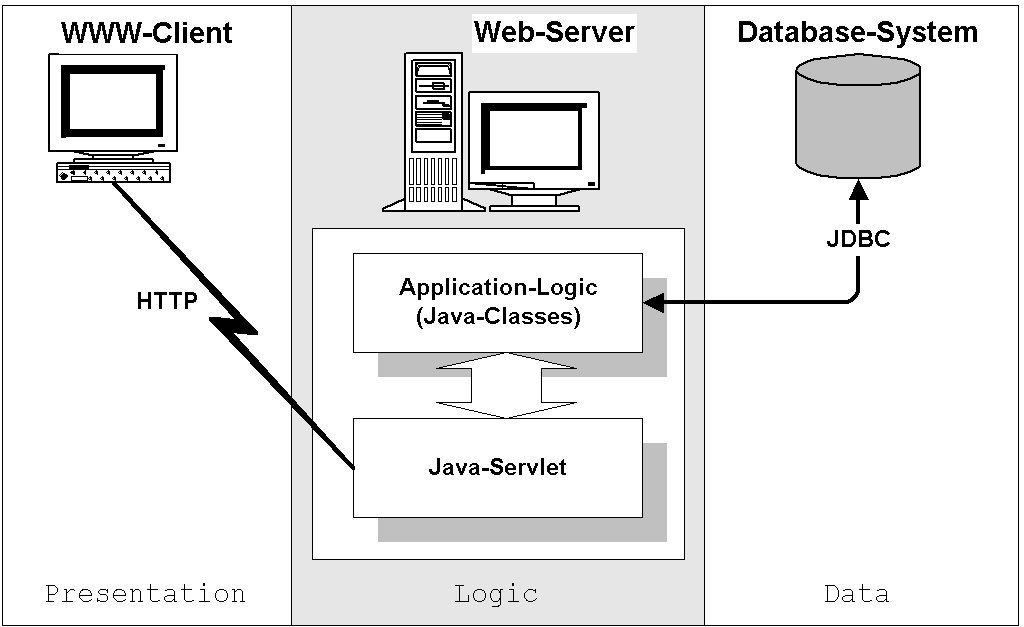
\includegraphics[clip,width=\sgw]{pics/modules/1}
\end{center}
\caption[3-tier-achitecture]{Example of a 3-tier-architecture using OpenCms}
\label{3-tier1}
\end{figure}

The presentation layer consists of a web browser (Internet Explorer or
Netscape Navigator) that is used to display an navigate through the HTML
user interface. Regardless of the browser used, it must be Version 4 or
higher. If you use an older version of the browser you will not be able
to execute the existing DHTML functions (JavaScript code) or attach
external style sheets. Both are necessary for a correct  usage of the
application.

The logic layer lies on the web server, which is extended by a runtime
environment for Java servlets. The web server can be the Apache web
server (Version 1.3.6 or higher), the configuration of which must be
completed by the so called "Jserv module" (the Servlet Engine,
Version 1.0 or higher), in order to execute servlets. All Java classes
are installed in the servlet environment on the server.
The OpenCms servlet (one single class) provides the interface to the
presentation layer as well as the interface to the database layer. It
uses the HTTP protocol to establish the communication between the
client and the application on the server (in this case OpenCms).
The database is accessed through the JDBC interface. The database
contains tables for resource, user and property data.

The following figure shows the most important components of OpenCms 
(Figure~\ref {Components}).\\

\begin{figure}
\begin{center}
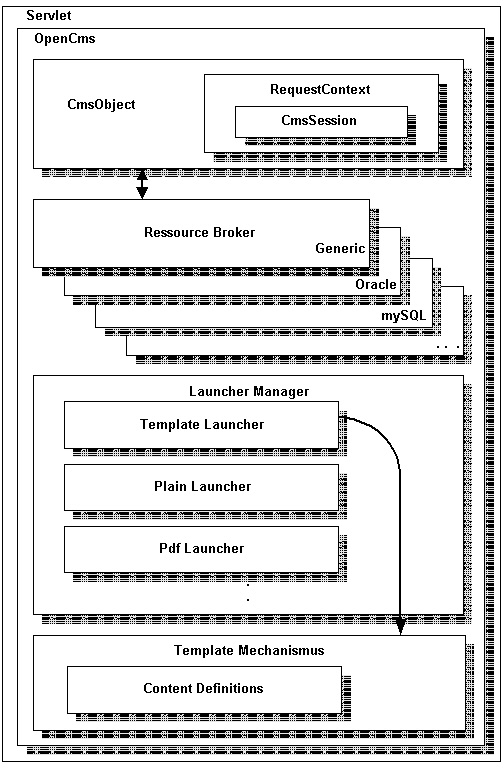
\includegraphics[clip,width=0.7 \linewidth]{pics/modules/2}
\end{center}
\caption[Components]{Compoments}
\label{Components}
\end{figure}


{\bf CmsObject:}
All resources are accessed via the \index{CmsObject} CmsObject. This is the interface to
the OpenCms system for the Module Developer. The CmsObject is
initialized with the user data.

{\bf Resource Broker:}
The \index{resource broker} resource broker checks requests for resources and performs them if
the user has the appropriate access permissions. It's configuration
depends on the database that is used.

{\bf Launcher Manager:}
The \index{Launcher Manager} Launcher Manager determines the launcher that will generate the
output with the requested content based on the type and/or content of
the selected file. If the template launcher has been selected, the
Template Mechanism is started.

{\bf Template Mechanism:}
The \index{Template Mechanism} Template Mechanism creates HTML pages based on the content in its
structured form. Content definitions enable you to access content that
originates from different sources (e.g. Virtual File System (VFS),
database, file system ...).


\subsection{Accessing system resources}
The general procedure of requesting an OpenCms web page is shown in the
next figure. First, a request is sent from the web browser. The URL
contains the host, the servlet path and the URI. The web server starts
the \index{servlet engine} servlet engine because the URI is within the servlet path, enabling
the servlet engine to pass it to OpenCms (Figure~\ref {Accessing1}).

\begin{figure}
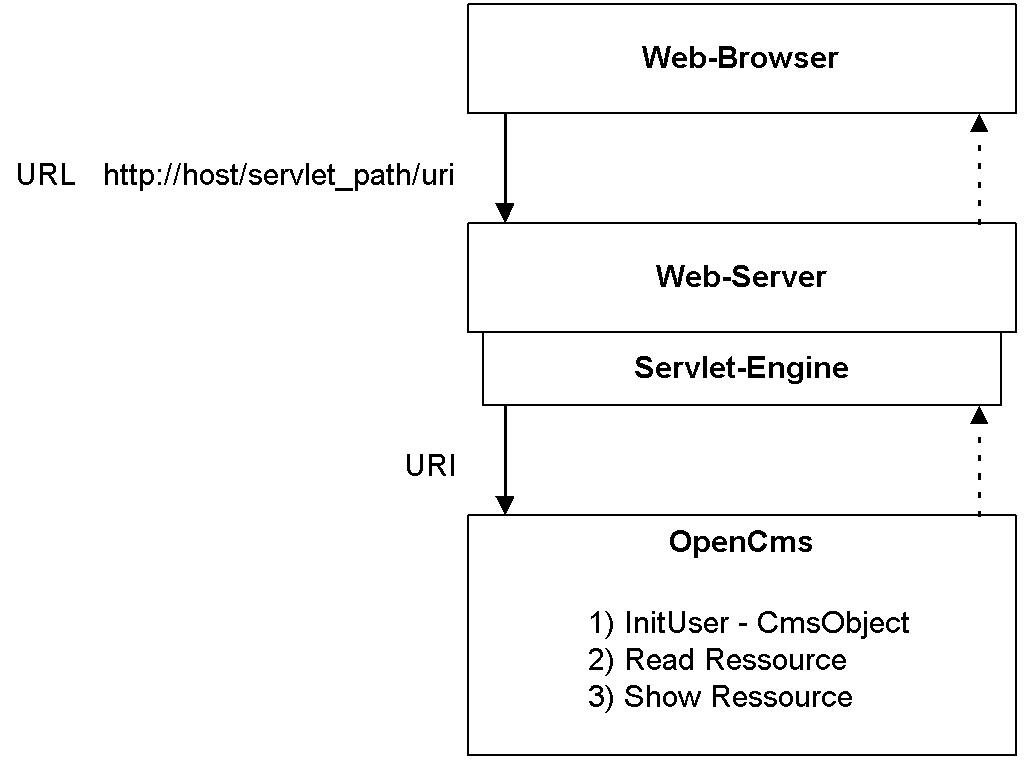
\includegraphics[clip,width=\sgw]{pics/modules/3}
\caption[Accessing system resources]{Accessing system resources}
\label{Accessing1}
\end{figure}

System resources are accessed via an instance of the class {\name CmsObject},
which provides the public interface that is used to access the system
and create the corresponding context. From the {\name msObject}, requests are
forwarded to the non-public parts of OpenCms. Thus, an instance of the
class {\name CmsObject} is created and initialized with the current user first.
The{\name CmsObject} passes the resource request to the resource broker. The
{\name resource broker} is the interface to the database. It performs the
request via the database access module and returns the resource if the
user has the right to access it. The access module establishes the
connection between the logic layer (application) and the database layer.
If a resource is requested, the {\name resource broker} forwards the request to
the access module. The access module generates an SQL statement to get
the data from the database. It then generates a {\name CmsRessourcObject} from
the database data and returns it to the resource broker. The {\name resource
broker} can now check the access permissions of the file and return the
file to the {\name CmsObject} providing the user has the appropriate access
permissions.

Because OpenCms works with different kinds of databases, the {\name resource
broker} and the access module are configured according to the used
database (Oracle, mySQL, etc.).
\index{database}
The following figure shows the structure used to access resources (figure~\ref {Accessing2}).

\begin{figure}
\begin{center}
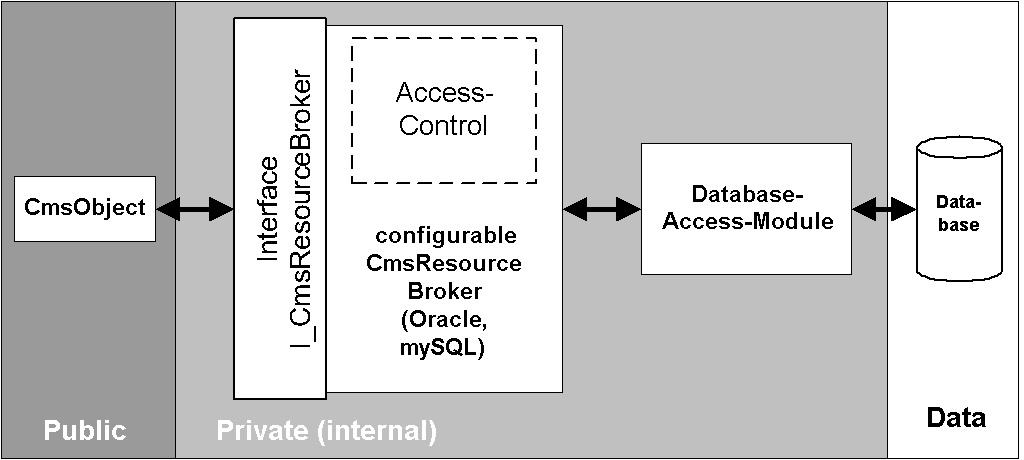
\includegraphics[clip,width=\sgw]{pics/modules/4}
\end{center}
\caption[Accessing resources in OpenCms]{Accessing resources in OpenCms}
\label{Accessing2}
\end{figure}

If the operation is successful (i.e. the user has permission to read
the file), the resource is displayed (sent to the user's web browser).

This is done by the {\name Launcher Manager}. The {\name Launcher Manager} starts a
certain launcher according to the type of the requested resource. For
pure text files, images etc. the plain launcher is used, which forwards
the content of the resource directly. The {\name template launcher} is used to
start the Template Mechanism when a template is requested. The {\name Template
Mechanism} creates HTML pages based on the content in its structured form.

The different launchers and the {\name Template Mechanism} will be explained in
detail in the following chapters.
\newpage

\subsection{Resources}
All of the Objects that are administrated in OpenCms are called
{\name resources}. At the moment, there are eight different types of
resources. With the exception of the resource type {\name folder,} all other
types are resources files that have content that can be displayed in a
browser. The  resource type is used to provide every file with aresources
processing instance - called {\name Launcher} - which starts the processing
process and then displays the data. The following table shows the
existing relationships. {Table~\ref {resources}}
\index{resource type}
\begin{table}[h]
\begin{center}
\begin{tabular}{|l|c|p{0.50\linewidth}|l|}
\hline
{\bf Name}& 
{\bf ID}& 
{\bf Description}& 
{\bf Launcher}\\ \hline
folder&
0& Folder&none\\ \hline
plain&
1&
Files that are notprocessed by OpenCms (text files, JavaScript libraries etc.)&
Dump launcher\\ \hline
XMLTemplate&
2&
XML coded template file.&
XML launcher\\ \hline
page&
3&
Representation of a whole site ("clickable file" or "page file").&
XML launcher\\ \hline
binary&
4& 
Binary files (like zip archives and PDF documents, but not graphics) that can be uploaded.&
Dump launcher\\ \hline
image& 
5& 
Binary graphic files (like  GIFJPEG& 
Dump launcher\\ \hline
script& 
6& 
Designed for JavaScript on the server- side& 
Dump launcher\\ \hline
newspage&
7& 
Representation of a news article, special caseof a page file& 
XML launcher\\ \hline 
\end{tabular}
\caption [Resources in OpenCms]{Resources in OpenCms}
\end{center}
\label{resources}
\end{table}

\subsection{The Virtual File System (VFS) of OpenCms}
\index{Virtual File System}
\index{VFS}
All of the files and folders of the different projects that are
displayed in the Explorer view that is part of the OpenCms Workplace,
are not stored in the normal file system. OpenCms has a {\name Virtual File
System} that holds the files and folders in a database, and an integrated
access permission administration. The access permissions in OpenCms are
similar to those of the UNIX file system. However, by using a {\name VFS} and a
database, OpenCms is independent from the operating system that is
installed on the server. In this way OpenCms can run on a Windows 95/98
system, which itself has no access permission administration at all.
Here is a short overview of the folders and the files in the standard
OpenCms {\name Virtual File System:} {Table~\ref {VFS}}

\begin{table}
\begin{center}
\begin{tabular}{|l|p{0.55\linewidth}|}
\hline
{\bf Directory}&
{\bf Files located in the directory}\\ [0.5ex] \hline
{\dir /content}&
Parent directory of  the directories that store the template files.\\ \hline
{\dir /content/bodys}&
Body templates are stored in this directory or a subdirectory thereof. They are stored in a directory with the same name
as the directory in which the web site is located.\\ \hline
{\dir /content/internal}&
Templates (subtemplates) that are not body  or master templates.\\ \hline
{\dir /content/templates}&
The master templates that define the general layout of a web site.\\ \hline
{\dir /download}&
Subdirectories for files that can be downloaded (galleries).\\ \hline
{\dir /pics}&
Subdirectories for pictures that are used in web sites (galleries).\\ \hline
{\dir /system}&
Parent directory of the directories that contain workplace templates and configuration files for the system.\\ \hline
{\dir /system/workplace/action}&
Executable files like login, copy etc.\\ \hline
{\dir /system/workplace/administration}&
Subdirectories for every Item in the Administration view.\\ \hline
{\dir /system/workplace/config}&
The language files, that are stored in a separate subdirectory for every language, and  the different
configuration files.\\ \hline
{\dir /system/workplace/css}&
Used style sheets.\\ \hline
{\dir /system/workplace/help}&
The help system.\\ \hline
{\dir /system/workplace/pics}&
The pictures that are used to create the workplace.\\ \hline
{\dir /system/workplace/templates}&
The templates that are used to create the workplace.\\ \hline
\end{tabular}
\caption [VFS of OpenCms]{VFS of OpenCms}
\label{VFS}
\end{center}
\end{table}

\subsection{Class structure}
The functionality of OpenCms is implemented in many different Java
classes. The classes are divided into different packages to structure
the code. Currently, there are 10packages that  cover a certain part
of the system's functionality.{Table~\ref {Classtruc}}

\begin{table}[h]
\begin{center}
\begin{tabular}{|l|p{0.55\linewidth}|}
\hline
{\name com.opencms.core}&
Classes of the system's core. The package also contains the OpenCms servlet.\\ \hline
{\name com.opencms.file}&
Definitions of all of the objects. \\ \hline
{\name com.opencms.file.genericSql}&
Resource broker for generic SQL databases. \\ \hline
{\name com.opencms.file.mySql}&
Special resource broker for mySQL.\\ \hline
{\name  com.opencms.file.oracleplsql}&
Special resource broker for ORACLE.\\ \hline
{\name com.opencms.file.utils}&
File package.\\ \hline
{\name com.opencms.launcher}&
All of the launchers that are used to display files or templates and a Launcher Manager.\\ \hline
{\name com.opencms.template}&
All of the template classes that are used to create documents dynamically and a Template Manager.\\ \hline
{\name com.opencms.util}&
Some general functionality (encoder, decoder etc.)\\ \hline
{\name com.opencms.workplace}&
All of the components (e.g. buttons, context-sensitive menus etc.) and functions (e.g. create project) of
the user interface (OpenCms Workplace).\\ \hline

\end{tabular}
\caption [Class structure]{Class structure}
\label {Classtruc}
\end{center}
\end{table}

\section{The template mechanism}
\subsection{Defining the Content of Data Blocks Dynamically}
We do already now how data blocks are used in templates.
In this example we will define the content of the data block in a Java
method. That means we will write our own class that controls the output
of the template and is places the text in the data block. To place
something in a data block that can dynamically be changed we will use
the {\tag <PROCESS>} tag inside of the data block.
Here is the content of the master template file:

\begin{xml}
<?xml version="1.0"?>\\
<XMLTEMPLATE>\\
<TEMPLATE>\\
\xtaba  <![CDATA[\\
\xtaba  <HTML>\\
\xtabb    <HEAD>\\
\xtabb    <TITLE>]]><method name="getTitle"/><![CDATA[</TITLE>\\
\xtabb    </HEAD>\\
\xtabb    <BODY>\\
\xtabb    ]]><ELEMENT name="body"/><![CDATA[\\
\xtabb    </BODY>\\
\xtaba  </HTML>\\
\xtaba  ]]>\\
</TEMPLATE>\\
</XMLTEMPLATE>\\
\end{xml}

The master template, which contains the framework of the HTML page, and
the data block will now be inserted in the body template. The body
template is automatically created when you create a new page. Body
templates have the same name as the page and are stored in the
{\dir /content/body} directory. If you look at the created file by going to
the{\dir /content/body} directory and selecting {\name Edit Code} you will see that
the generated template contains the absolute minimum framework of a
template:

\begin{xml}
<?xml version="1.0"?>\\
<XMLTEMPLATE>\\
<TEMPLATE/>\\
</XMLTEMPLATE>\\
\end{xml}

We will now change the content of the body template and add a data
block and process tag. The new body template should contain the
following text:

\begin{xml}
<?xml version= "1.0 "?>\\
<XMLTEMPLATE>\\
<MESSAGE>\\
<![CDATA[Hello, World ]]>\\
<PROCESS>greeting</PROCESS>\\
</MESSAGE>\\
\end{xml}

\begin{xml}
<TEMPLATE>\\
<PROCESS>message</PROCESS>\\
</TEMPLATE>\\
</XMLTEMPLATE>\\
\end{xml}

Edit the file and close the editor by clicking on  the {\name Save and Exit}
icon. Create a new empty page in the root directory that will use the
new template.
The next step is to write the Java class that controls the output of
our new template. The new class will be derived from the {\class CmsXmlTemplate}
class. This class provides the basic functionality to control template
files. In the new class we will override the {\meth getContent()} method. This
method is creates the output of the template and is invoked
automatically by the OpenCms system. Inside this method we will use the
{\meth setData()} method to replace the {\tag <PROCESS>} greeting {\tag</PROCESS>}
construction.

This is the source code for our new class:

\begin{java}
import com.opencms.template.*;\\
import com.opencms.file.*;\\
import com.opencms.core.*;\\

import java.util.*;\\

public class CmsExample4 extends CmsXmlTemplate \{\\
\index{getContent}
public byte[] getContent(CmsObject cms,\\
\jtabd        String templateFile, String elementName,\\
\jtabd        Hashtable parameters,String templateSelector)\\
\jtabd        throws CmsException \{\\
\jtabe        CmsXmlTemplateFile templateDocument =\\
\jtabe        getOwnTemplateFile(cms, templateFile, elementName,\\
\jtabf                           parameters,templateSelector);\\


\jtabe        templateDocument.setData("greeting","from Java!");\\
\jtabe        return startProcessing(cms,\\
\jtabe                               templateDocument, elementName,\\
\jtabe                               parameters, templateFile);\\
\jtabb    \}\\
\}\\
\end{java}

You can compile the class (on the console with: {\class javac Example4.java)}
and place the generated {\class Example4.class} in your servlet zone root
directory. Now we must tell the system that this class should be used
to control the template output. This can be done by editing the page
{\name control file}. The page {\name control file} can be accessed from the context
menu by selecting {\name Edit ControlCode} (figure~\ref{EditControlCode1}).

\begin{figure}
\begin{center}
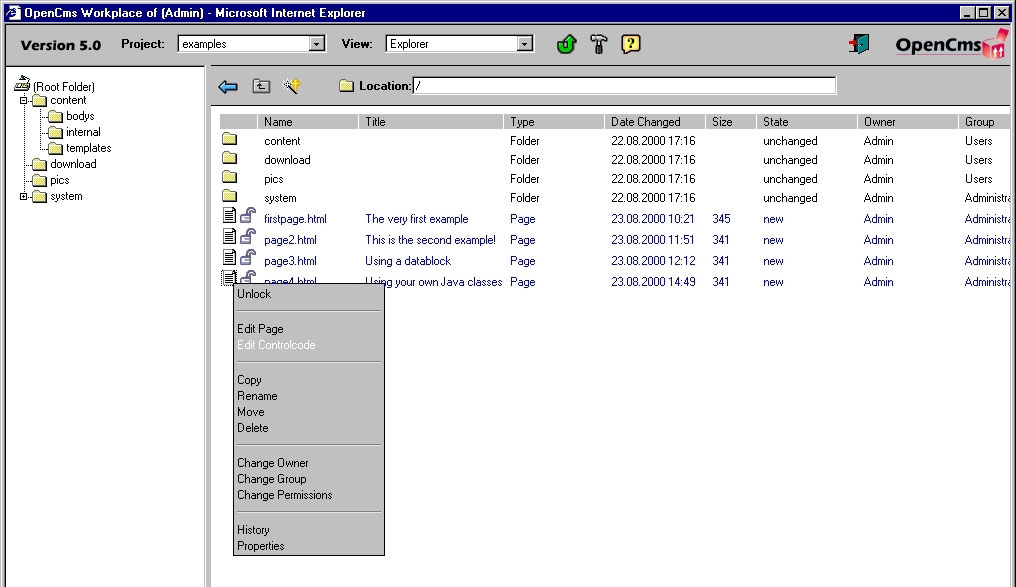
\includegraphics[clip,width=\sgw]{pics/modules/29}
\end{center}
\caption[EditControlCode1]{Select Edit ControlCode to edit the page control file.}
\label{EditControlCode1}
\end{figure}

The page will contain text that looks like this:

\begin{xml}
<?xml version= "1.0 " encoding= "ISO-8859-1 "?>\\
<page>\\
\xtaba <CLASS>com.opencms.template.CmsXmlTemplate</CLASS>\\
\xtaba <MASTERTEMPLATE>/content/templates/template4</MASTERTEMPLATE>\\
\xtaba <ELEMENTDEF name="body">\\
\xtaba <CLASS>com.opencms.template.CmsXmlTemplate</CLASS>\\
\xtaba <TEMPLATE>/content/bodys/page4.html</TEMPLATE>\\
\xtaba </ELEMENTDEF>\\
</page>\\
\end{xml}

You can see two {\tag <CLASS>} tags that define which Java classes will be
used to control the templates. The first entry is the one for the
master template and should always use the default
{\class com.opencms.template.CmsXmlTemplate} class. The second entry for a class
defines the class that controls the body template. This entry must be
changed, and the name of our new class ({\class CmsExample4}) should be placed
inside the {\tag <CLASS>} tag. If you have selected to add a package statement
in the classes source code you have to type the fully qualified class
name inside the{\tag <CLASS>} tag.
The page control file should look like this:

\begin{xml}
<?xml version= "1.0 " encoding= "ISO-8859-1 "?>\\
<page>\\
\xtaba <CLASS>com.opencms.template.CmsXmlTemplate</CLASS>\\
\xtaba <MASTERTEMPLATE>/content/templates/template4</MASTERTEMPLATE>\\
\xtaba <ELEMENTDEF name="body">\\
\xtaba <CLASS>CmsExample4</CLASS>\\
\xtaba <TEMPLATE>/content/bodys/page4.html</TEMPLATE>\\
\xtaba </ELEMENTDEF>\\
</page>\\
\end{xml}

Note that the name of the master template file and the body template
file will be different if you entered different names for your files.
When you have adjusted the {\name page control} file you can save it and leave
the editor.

Every time a new class has been placed in your servlet zone, you must
log out and restart the OpenCms system. If your server is configured to
autoreload classes in the servlet zone you should be able to work with
the new classes after you log in again. If this is not the case, it's
the best to shutdown and restart the server if you encounter any
unexpected server problems. When you have done this, you can click on
the new page to view it.
The result should look like figure~\ref{OutputJavaClass}.

\begin{figure}
\begin{center}
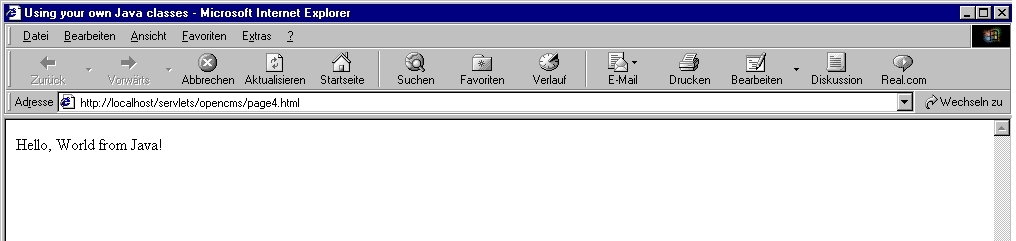
\includegraphics[clip,width=\sgw]{pics/modules/30}
\end{center}
\caption[Output generated using the new Java class]{Output generated using the new Java class}
\label{OutputJavaClass}
\end{figure}

\subsection{Using user-defined Methods}
In the last example we saw one way of creating dynamic content in a
template. Another way is to use user-defined methods in the template.
You have already seen how to use the {\meth getTitle(}) method in a template in
the second example. If you want to write your own methods, you can
derive a class from the existing template class
{\class com.opencms.template.Cms\-Xml\-Template} and add your own methods.

The master template should contain the following text:

\begin{xml}
<TEMPLATE>\\
\xtaba  <![CDATA[\\
\xtaba  <HTML>\\
\xtabb    <HEAD>\\
\xtabb    <TITLE>]]><method name="getTitle"/><![CDATA[</TITLE>\\
\xtabb    </HEAD>\\
\xtabb    <BODY>\\
\xtabb    ]]><ELEMENT name="body"/><![CDATA[\\
\xtabb    </BODY>\\
\xtaba  </HTML>\\
\xtaba  ]]>\\
</TEMPLATE>\\
</XMLTEMPLATE>\\
\end{xml}

This template defines the title of the page and inserts a body element.
The method tag can be placed in the body template. We will write a
method that returns the string {\name Hello, World from Java} and give it the
name{\meth getHello(}). The result will be the same as that of the previous
example: the text will be inserted in the output of the page. The body
template should contain the following:

\begin{xml}
<?xml version="1.0"?>\\
<XMLTEMPLATE>\\
<TEMPLATE>\\
<METHOD name="getHello"/>\\
</TEMPLATE>\\
</XMLTEMPLATE>\\
\end{xml}

A new Java class {\class CmsExample5} defines the method {\meth getHello(}):

\begin{xml}
import com.opencms.template.*;\\
import com.opencms.file.*;\\
import com.opencms.core.*;\\


import java.util.*;\\

public class  CmsExample5 extends  CmsXmlTemplate \{\\

\xtabb   public Object getHello(CmsObject cms, String tagcontent,\\
\xtabd           A\_CmsXmlContent doc, Object userObject) \{\\
\xtabc       return "Hello, World from Java!";\\
\xtabb   \}\\

\}\\
\end{xml}

To use the class, compile it and place it in your servlets directory.
Create a new page that uses the master template that was created at the
beginning of this section, and edit the page control file (use {\name Edit
Controlcode} in the context menu). Now you have to change the class
that controls the body template. The page {\name control file} should look like
this:

\begin{xml}
<?xml version= "1.0 "?>\\
<page>\\
\xtaba <CLASS>com.opencms.template.CmsXmlTemplate</CLASS>\\
\xtaba <MASTERTEMPLATE>/content/templates/template5</MASTERTEMPLATE>\\
\xtaba <ELEMENTDEF name="body">\\
\xtaba <CLASS>CmsExample5</CLASS>\\
\xtaba <TEMPLATE>/content/bodys/page5.html</TEMPLATE>\\
\xtaba </ELEMENTDEF>\\
</page>\\
\end{xml}

The output of the new template will be the same as that of the previous
example: it displays the string {\name Hello, World from Java!} on the screen.
The only difference is the procedure we followed to accomplished the
task of inserting something in the document. In the previous example we
replaced the process tag with the {\meth setData()} method and now we used the
entirely new method {\meth getHello()}.

\subsection{Details of OpenCms Template Programming}
\subsubsection{The relationship between Templates, Page Control Files, and
Java Classes}

For every new page that is created with OpenCms, the system
automatically creates a page control file. This {\name page control file}
determines the templates that are used by the new page and the Java
classes that are used to control them. Examples for page control files
have already been shown before. The different entries in these files
will be explained in the following section.
Below is the page control file for an earlier example:

\begin{xml}
<?xml version= "1.0 "?>\\
<page>\\
\xtaba <CLASS>com.opencms.template.CmsXmlTemplate</CLASS>\\
\xtaba <MASTERTEMPLATE>/content/templates/template5</MASTERTEMPLATE>\\
\xtaba <ELEMENTDEF name="body">\\
\xtaba <CLASS>CmsExample5</CLASS>\\
\xtaba <TEMPLATE>/content/bodys/page5.html</TEMPLATE>\\
\xtaba </ELEMENTDEF>\\
</page>\\
\end{xml}

As can be seen in the first line this file is an XML document. There
are two {\class <CLASS>} entries and two entries for templates. The first
template entry is the one for the master template and the second is for
the body template. The name of the master template file is enclosed
between {\tag <MASTERTEMPLATE>} tags. The {\tag <CLASS>} tag above it determines the
Java class that controls the master template. This class is the  generic
{\class com.opencms.template.CmsXmlTemplate} class and should always be used to
control the master template. The {\tag <ELEMENTDEF>} tag defines an element
with the name {\name body.} An element definition must be provided for every
subelement (subtemplate) that is inserted in the document. The body
element can be placed in the master template with the element tag as
follows:

{\tag <ELEMENT name="body"/>}

You can place other subtemplates in your document in the same way you
placed the body template in it, by inserting a
{\tag <ELEMENT name="aNewName"/>} tag and element definition in your document.
The name for the new element can be freely defined.
The controlling Java class for the body template can be one of the
existing template classes or one that is derived from these classes and
defined by you. In the example above we used the {\class CmsExample5} class,
which defined the new method {\meth getHello()}.


\subsubsection{The Difference between the Master and the Body Template}
The master template is the template that holds the body template and
all of its subtemplates. The master template mainly defines the layout
of the whole page and the gaps in which the templates are inserted.
The following graphic shows the structure of a typical web site created
with OpenCms (figure~\ref{DiffMasterBodyTemp}).

\begin{figure}
\begin{center}
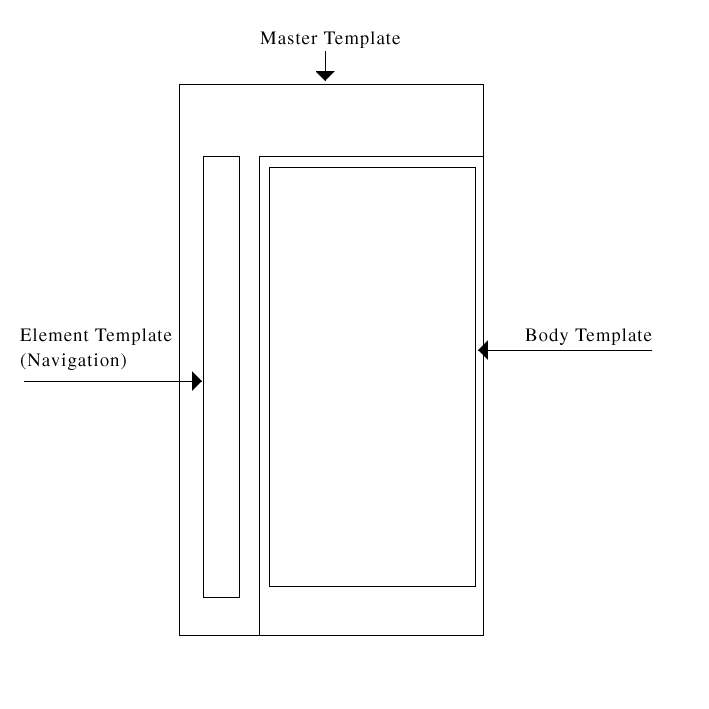
\includegraphics[clip,width=\sgw]{pics/modules/31}
\end{center}
\caption[Structure of a typical OpenCms web side]{Structure of a typical OpenCms web side.}
\label{DiffMasterBodyTemp}
\end{figure}

The master template in this graphic contains a body template and an 
{\class {CmsXmlFormTemplateFile}}
element template (subtemplate) that creates the navigation. The body
template and all of the other element templates are also capable of
containing subtemplates. This enables you to structure your document in
any imaginable way. The master template and the subtemplates can easily
be reused for the design of other web sites.

\subsubsection{Process, Method and Element Tags}
The process, {\tag method} and {\tag element} tags enable you to insert dynamic
content in your web site. They have already been used in the first
examples. Their syntax and their usage will be discussed in the
following sections.

\subsubsection{The Process Tag}
The {\tag process} tag can be used to insert the content of data blocks in
your document. The data blocks can be defined in the document or set by
Java classes. We will explain how a process tag works by taking a look
at the second example of chapter 2.
Here is the content of the master template of this example:

\begin{xml}
<?xml version= "1.0 "?>\\
<XMLTEMPLATE>\\
<MESSAGE>\\
<![CDATA[Hello, World ]]>\\
<PROCESS>greeting</PROCESS>\\
</MESSAGE>\\

<TEMPLATE>\\
<PROCESS>message</PROCESS>\\
</TEMPLATE>\\
</XMLTEMPLATE>\\
\end{xml}

There are two process tags in this template: the first inside the data
block "message" and the second inside the template tag. The text inside
the process tag defines the data block that will be processed. In this
example two data blocks will be processed, one named "greeting" and one
named "message." The "message" data block is defined in the template
document. The data block "greeting" is not defined in the document, but
set in the Java class that is associated with the template. The
{\meth setData()} method was used to accomplish this:

{\meth templateDocument.setData("greeting","from Java!");}

This way the data block can be set dynamically in the Java classes. To
show that it is possible to set the data block randomly inside a Java
class, the next examples insert a randomly selected link to a web site.
This is the content of the body template file:

\begin{xml}
<?xml version="1.0"?>\\
<XMLTEMPLATE>\\
<LINK1>www.opencms.org</LINK1>\\
<LINK2>www.yahoo.de</LINK2>\\
<TEMPLATE>\\
<![CDATA[\\
<a href="http://]]><PROCESS>link</PROCESS><![CDATA[">\\
Where will we go?</a>\\
]]>\\
</TEMPLATE>\\
</XMLTEMPLATE>\\
\end{xml}

The master template creates a web site with a {\name body} element:

\begin{xml}
<?xml version="1.0"?>\\
<XMLTEMPLATE>\\
<TEMPLATE>\\
\xtaba <![CDATA[\\
\xtaba <HTML>\\
\xtaba <HEAD>\\
\xtaba <TITLE>]]><method name="getTitle"/><![CDATA[</TITLE>\\
\xtaba </HEAD>\\
<BODY>\\
\xtaba ]]><ELEMENT name="body"/><![CDATA[\\
\xtaba </BODY>\\
\xtaba </HTML>\\
\xtaba ]]>\\
</TEMPLATE>\\
</XMLTEMPLATE>\\
\end{xml}

The target of the link will be set randomly in a Java class.
This is the source code for the new class:

\begin{java}
import com.opencms.template.*;\\
import com.opencms.file.*;\\
import com.opencms.core.*;\\
import java.util.*;\\[1ex]


public class CmsExample6 extends CmsXmlTemplate \{\\[1ex]

\jtaba public byte[] getContent(CmsObject cms,\\
\jtabc        String templateFile, String elementName,\\
\jtabc        Hashtable parameters,String templateSelector)\\
\jtabc        throws CmsException \{\\
\jtabb   String linkTarget;\\
\jtabb   linkTarget = "LINK"\\
\jtabd       + String.valueOf((int)(Math.random()*2+1));\\
\jtabb   CmsXmlTemplateFile templateDocument =\\
\jtabd       getOwnTemplateFile(cms, templateFile, elementName,\\
\jtabd       parameters,templateSelector);\\
\jtabb   templateDocument.setData("link",\\
\jtabd       templateDocument.getDataValue(linkTarget));\\
\jtabb   return startProcessing(cms, templateDocument, elementName,\\
\jtabd       parameters, templateFile);\\
\jtaba \}\\[1ex]

\jtaba public CmsCacheDirectives getCacheDirectives(CmsObject cms,\\
\jtabd     String templateFile, String elementName,\\
\jtabd   Hashtable parameters, String templateSelector) \{\\
\jtabb   return new CmsCacheDirectives(false);\\
\jtabb \}\\
\}\\
\end{java}
\index{getCacheDirectives()}
\index{CmsCacheDirectives}

The data block that is used for link's target is randomly selected in
the line:

\begin{java}
linkTarget = "LINK"\\
\jtabd              + String.valueOf((int)(Math.random()*2+1));\\
\end{java}

This statement produces a string {\name "Link1"} or {\name "Link2"} based on the number
that is randomly created by the expression {\name (Math.random()*2+1)}.
The data block link is defined in the following expression:

{\code templateDocument.setData("link",\\
  templateDocument.getDataValue(linkTarget));}

The data block named {\name "link"} is defined with the method {\meth setData()} and
the content of the data block is the value of the data block that will
be fetched with {\meth getDataValue(linkTarget)}. Because the variable
{\name linkTarget} has either the value {\name "Link1"} or {\name "Link2"} the link will be
defined with the content of data block {\name "Link1"} or{\name  "Link2"}.
To ensure that the link is refreshed every time the page is requested,
the class overrides the method {\meth getCacheDirectives()}. This method controls
the way elements are cached in OpenCms. The implementation in the superclass
{\class CmsXmlTemplate} uses the caching mechanism and would prevent the element
from being refreshed every time it is requested. The details of the element caching mechanism 
are explained on page \pageref{element cache}.
At this point it is only necessary to know that if an element should be dynamically created
on every request the method {\meth getCacheDirectives} has to be implemented in the template class
in the way we did in this example.


The next example will show how to create tables or lists using the
{\tag process} tag. You can use the {\tag process} tag to set the data entries in
tables in Java classes. The table will be dynamically built in the Java
class by producing a string that concatenates the table rows. The
layout of the table is defined in the template. For this example, we
can use the master template that was used in the previous example: an
empty site with a body element. However, if you want you can create a
new page and select the master template that was used in {\name example 7.} The
whole layout will be defined in the body template. This is the content
of the body template:

\begin{xml}
<?xml version="1.0"?>\\
<XMLTEMPLATE>\\

<TEMPLATE>\\
<![CDATA[ <H1>Animal list</H1>\\
<table border=1>\\
]]>\\
<process>tablehead</process>\\
<process>list</process>\\
<![CDATA[\\
</table>\\
]]>\\
</TEMPLATE>\\
<tablehead>\\
<![CDATA[\\
<tr>\\
<td>Nr</td>\\
<td>animal</td>\\
<td>owner</td>\\
</tr>\\
]]>\\
</tablehead>\\
<row>\\
<![CDATA[\\
<tr>\\
<td>]]><process>number</process><![CDATA[</td>\\
<td>]]><process>name</process><![CDATA[</td>\\
<td> ]]><process>owner</process><![CDATA[</td>\\
</tr>\\
]]>\\
</row>\\
</XMLTEMPLATE>\\
\end{xml}


The template defines a table and two data blocks. The data block
{\tag "tablehead"} defines a static heading for every column and will be
inserted in the table by the {\tag process} tag. The content of the table will
be created in a Java class and will be set as the data block {\name list.}
The layout table's rows is defined by the data block {\name row.} The Java
class will set the content of every row, concatenate the results and
insert them in the document as the data block {\name list.} Here is the
source code of the Java class:

\begin{java}
import com.opencms.file.*;\\
import com.opencms.template.*;\\
import java.util.*;\\

public class CmsExample7 extends CmsXmlTemplate \{\\
public byte[] getContent(CmsObject cms, String templateFile,\\
\jtabc        String elementName, Hashtable parameters,\\
\jtabc        String templateSelector) throws CmsException \{\\
\jtabb    String[] owners =\\
\jtabc       {"Martin","Thomas","Andreas","Bill","Michael","Doris"};\\
\jtabb    String[] animals =\\
\jtabc       {"cat","dog","mouse","rat","bird","snake"};\\
\jtabb    CmsXmlTemplateFile template =\\
\jtabd        getOwnTemplateFile(cms,templateFile,elementName,\\
\jtabd        parameters,templateSelector);\\
\jtabb    String list = "";\\
\jtabb    for (int i=0; i < animals.length;  i++) \{\\
\jtabd        template.setData("number",i+"");\\
\jtabd        template.setData("name",animals[i]);\\
\jtabd        template.setData("owner",owners[i]);\\
\jtabd        String row = template.getProcessedDataValue("row");\\
\jtabe           list += row;\\
\jtabb    \}\\
\jtabb    template.setData("list",list);\\
\jtabb    return startProcessing(cms, template, elementName,\\
\jtabd        parameters, templateSelector);\\
\jtabb    \}\\
\}\\
\end{java}
\index{CmsXmlTemplateFile}
\index{getOwnTemplateFile}
The Java class overrides the method {\meth getContent()} that creates the
template's output. Two string arrays are defined in this method that
hold the entries for the owners and the animals that will be inserted
in the table. The rows are generated by setting the data blocks
{\name number} , {\name name}, and {\name owner} in the data block  {\name row} and fetching the
processed data block {\name row} (this means the process tags have been
replaced by the corresponding data blocks). The result is concatenated
in a string and set as the data block {\name list.} The final call to
{\code startProcessing()} starts the generation of the template's output.
The last example can be modified to produce a list instead of a table.
The Java class can be left unchanged and reused to create the list.
This shows that it is possible to change the layout in the template
without having to change the Java class. This is the template that will
generate a list instead of a table:

\begin{java}
<?xml version="1.0"?>\\
<XMLTEMPLATE>\\

<TEMPLATE>\\
<![CDATA[ <H1>Animal list 2</H1>\\
<ul>\\
\jtabb    ]]>\\
\jtabb    <process>list</process>\\
\jtabb    <![CDATA[\\
</ul>\\
]]>\\
</TEMPLATE>\\
<row>\\
<![CDATA[\\
<li>\\
]]><process>name</process><![CDATA[,\\
]]><process>owner</process><![CDATA[\\
</li>\\
]]>\\
</row>\\
</XMLTEMPLATE>\\
\end{java}

The template places the data block "list" in an unsorted list. The
rows' layout has been changed to list entries. The name and the owner
are set in the Java class and the list is generated in the same way
that it was in the last example. Note that the data block number is not
used by the template, but still set in the Java class. Although this is
redundant, it is harmless because the data block is set without being
processed.

\subsubsection{The Method Tag}
The method tag is used to insert the output of a method in a document.
You can use a new method that is defined in a class that is derived
from one of the existing template classes or a standard method that is
defined by the existing classes. In the last example of Chapter 2 we
created the new method {\meth getHello()}to show how method tags are used.
In general, a method is used in a template by inserting a method tag.
A method can take parameters that are passed to the method by
specifying them in the method tag.

The syntax for the method tag:

{\meth - <method name="test"/>

- <method name="test2">parameter(s)</method>}

The method tag can be used in two ways: for methods that don't need any
parameters, the end tag {\tag </method>} can be omitted and the tag can be
closed by entering {\tag />}. When parameters are passed as a string to a
method in the tag, the method tag has to be closed with the
corresponding end tag {\tag (</method>)}.The examples that generated a table
and a list using a process tag can easily be modified to use a method
instead. The next example will show how to generate a table with the
new method {\meth getTable()}. Here is the body template:

\begin{xml}
<?xml version="1.0"?>\\
<XMLTEMPLATE>\\

<TEMPLATE>
<![CDATA[ <H1>Animal list</H1>\\
<table border=1>\\
]]>\\
<process>tablehead</process>\\
<method name="getTable"/>\\
<![CDATA[\\
</table>\\
]]>\\
</TEMPLATE>\\
<tablehead>\\
<![CDATA[\\
<tr>\\
<td>Nr</td>\\
<td>animal</td>\\
<td>owner</td>\\
</tr>\\
]]>\\
</tablehead>\\
<row>\\
<![CDATA[\\
<tr>\\
<td>]]><process>number</process><![CDATA[</td>\\
<td>]]><process>name</process><![CDATA[</td>\\
<td> ]]><process>owner</process><![CDATA[</td>\\
</tr>\\
]]>\\
</row>\\
</XMLTEMPLATE>\\

To insert the table in the document using a method rather than a\\
process tag, we modified the line\\

<process>list</process>\\

to\\

<method name="getTable"/>\\
\end{xml}

The table will be generated in a method. This is the Java source code:

\begin{java} 
import com.opencms.template.*;\\

import com.opencms.file.*;\\

import com.opencms.core.*;\\

import java.util.*;\\
public class CmsExample9 extends CmsXmlTemplate \{\\
\jtabb   public Object getTable(CmsObject cms, String tagcontent,\\
\jtabe           A\_CmsXmlContent doc, Object userObject)\\
\jtabe           throws CmsException \{\\
\jtabb   String[] owners =\\
\jtabc    {"Elmar","Randolf","Sandra","Geoffrey","Claudia","Doris"};\\
\jtabb   String[] animals =\\
\jtabc    {"spider","eagle","lion","cheetah","scorpion","snake"};\\
\jtabb   CmsXmlTemplateFile template = (CmsXmlTemplate)doc;\\
\jtabb   String list = "";\\
\jtabb   for (int i=0; i < animals.length;  i++) \{\\
\jtabd        template.setData("number",i+"");\\
\jtabd        template.setData("name",animals[i]);\\
\jtabd        template.setData("owner",owners[i]);\\
\jtabd        String row = template.getProcessedDataValue("row");\\
\jtabe           list += row;\\
\jtabb   \}\\
\jtabb   return list;\\
\jtabb   \}\\

\}\\
\end{java}

The names of the owners and the animals have been changed to emphasize
that this table is not the same as the one that was produced by using
the process tag.
To introduce another example of how methods can be used, we will take a
look at a method that returns a color value that can be inserted in an
HTML document. This method takes a parameter that defines the color
that should be used. The parameter consists of the string enclosed by
the method tag. The method will be used in the template as follows:

{\meth method name="color">red</method>}

The parameter will be used in the method to return the appropriate hex
number that represents the color. This number will be inserted in the
template to define the color that is used. This is the source code for
the new Java class and the method:

\begin{java}
import com.opencms.core.*;\\
import com.opencms.file.*;\\
import com.opencms.template.*;\\
import java.util.*;\\

public class CmsExample10 extends CmsXmlTemplate \{\\
\jtabc        static Hashtable colors = new Hashtable();\\
\jtabc        static \{\\
\jtabd                colors.put("black", "000000");\\
\jtabd                colors.put("maroon", "800000");\\
\jtabd                colors.put("green", "008000");\\
\jtabd                colors.put("olive", "808000");\\
\jtabd                colors.put("navy", "000080");\\
\jtabd                colors.put("purple", "800080");\\
\jtabd                colors.put("teal", "008080");\\
\jtabd                colors.put("gray", "0808080");\\
\jtabd                colors.put("silver", "C0C0C0");\\
\jtabd                colors.put("red", "FF0000");\\
\jtabd                colors.put("lime", "00FF00");\\
\jtabd                colors.put("yellow", "FFFF00");\\
\jtabd                colors.put("blue", "0000FF");\\
\jtabd                colors.put("fuchsia", "FF00FF");\\
\jtabd                colors.put("aqua", "00FFFF");\\
\jtabd                colors.put("white", "FFFFFF");\\
\jtabc        \}\\
\jtabb    public Object color(CmsObject cms, String tagcontent,\\
\jtabd            A\_CmsXmlContent doc, Object userObject)\\
\jtabd            throws CmsException \{\\
\jtabc        String color;\\
\jtabc        if (tagcontent == null || tagcontent.equals("")) \{\\
\jtabd            color = (String)colors.get("black");\\
\jtabc        \} else \{\\
\jtabd            color = (String)colors.get(tagcontent);\\
\jtabd            if (color == null) \{\\
\jtabd                color = (String)colors.get("black");\\
\jtabd            \}\\
\jtabc        \}\\
\jtabc        return "\#" + color;\\
\jtabb    \}\\
\}\\
\end{java}

As we can be see, a hash table is used to store the names of the colors
and the corresponding hexadecimal values. The method checks if a tag
content was passed to the method. If the tag content is passed, the
method tries to get the appropriate color value. If a the name of a
color is passed that is not contained in the hash table or if no tag
content is passed, the color black is used.

\subsubsection{Element Tag and Element Definition}
The element tag is used to insert subelements (subtemplates) in a web
site. The element definition defines the template and Java class that
are used for the element. In this section, we will take a look at the element tag
and element definition. The element tag must have the following syntax:

{\tag <ELEMENT name="aName"/>}

where {\name aName} must be replaced with the name of the element. A valid
element definition has the following structure:

\begin{xml}
<ELEMENTDEF name="aName">\\
<TEMPLATE>nameOfTheTemplateFile</TEMPLATE>\\
<CLASS>nameOfTheControllingClass</CLASS>\\
<PARAMETER name="param1">value1</PARAMETER>\\
<PARAMETER name="param2">value2</PARAMETER>\\
</ELEMENTDEF>\\
\end{xml}

In the element definition, the template file and the controlling Java
class are specified in the template and the class tag. It is also
possible to pass parameters to the controlling Java class. Parameters
that are specified in the element definition are accessible in the Java
class. They are stored in a hash table together with the parameters
that are appended to a URL.
The element definition is defined either in the document in which the
element is inserted, or in the page control file. If the element
definition is missing, the element definition of the element "body"
will be used. This element definition is automatically generated by the
system when a new page is created, but can be modified, for example, to
change the controlling Java classes. The element definition can also be
overridden in the page control file. If an element definition is
specified in both the file in which the element is inserted and in the
page control file, the element definition stored in the page control
file takes precedence. This means that the page control file can be
used to modify a default element definition.
The next example will show the effect of overriding element definitions.
First we need to create a template that contains elements that consist
of templates using data from the previous examples. This is the master
template for the new page:

\begin {xml}
<?xml version="1.0"?>\\
<XMLTEMPLATE>\\
<TEMPLATE>\\
<![CDATA[\\
<HTML>\\
<HEAD>\\
<TITLE>]]><method name="getTitle"/><![CDATA[</TITLE>\\
</HEAD>\\
<BODY>\\
<TABLE border width="100\%" height="100\%">\\
\xtaba        <TR height="30\%">\\
\xtabb                <TD width="20\%"><IMAGE src="\\
]]><method name="getServletPath"/><![CDATA[\\
pics/opencmslogo.gif" align="center">\\
</TD
\xtabb                <TD width="80\%" align="center"\\
]]><element name="hello"/><![CDATA[\\
</TD>\\
\xtaba        </TR>\\
\xtaba        <TR height="70\%">\\
\xtabb                <TD width="20\%" align="center" valign="top">\\
\xtabc                        ]]><element name="random"/><![CDATA[\\
\xtabb                </TD>\\
\xtabb                <TD width="80\%" align="center">\\
\xtabb                ]]><element name="body"/><![CDATA[\\
\xtaba        </TD>\\
\xtaba        </TR>\\
</TABLE>\\
</BODY>\\
</HTML>\\
]]>\\
</TEMPLATE>\\

<ELEMENTDEF name="hello">\\
<TEMPLATE>/content/bodys/page4.html</TEMPLATE>\\
<CLASS>CmsExample4</CLASS>\\
</ELEMENTDEF>\\

<ELEMENTDEF name="random">\\
<TEMPLATE>/content/bodys/page6.html</TEMPLATE>\\
<CLASS>CmsExample6</CLASS>\\
</ELEMENTDEF>\\

</XMLTEMPLATE>\\
\end{xml}

The template defines a table with two rows and two columns. A picture
of the  OpenCms logo is placed in the first row of the first column. An
element called {\name hello} is placed in the second column of the first row.
The corresponding element definition specifies this element as the one
we used in example 4: it displays the string {\name Hello, World from Java!}
on the screen.
The second row in the first column contains an element called {\name random.}
This element is the random link that we created in example 6. The body
element is inserted in the second column of row 2. This is the content
of the body template:

\begin{xml}
<?xml version="1.0"?>\\
<XMLTEMPLATE>\\
<TEMPLATE>\\
<![CDATA[\\
<TABLE border>\\
\xtaba        <TR>\\
<TD valign="top">\\
]]><element name="animaltable"/><![CDATA[\\
</TD>\\
\xtabb                <TD valign="top">\\
]]><elementname="animallist"/><![CDATA[\\
</TD>\\
\xtaba        </TR>\\
</TABLE>\\
]]>\\
</TEMPLATE>\\

<ELEMENTDEF name="animaltable">\\
<TEMPLATE>/content/bodys/page7.html</TEMPLATE>\\
<CLASS>CmsExample7</CLASS>\\
</ELEMENTDEF>\\

<ELEMENTDEF name="animallist">\\
<TEMPLATE>/content/bodys/page8.html</TEMPLATE>\\
<CLASS>CmsExample7</CLASS>\\
</ELEMENTDEF>\\

</XMLTEMPLATE>\\
\end{xml}

The body template defines a table with two elements that contain data
form previous examples: the table and a list of the animals and their
owners. When you look at the page you will see that the elements are
all placed in the document in the positions that are defined in the
template.
The effect of overriding an element definition will be shown in the
next example. An element definition is overridden by adding another
element definition in the page control file. This is the content of
the original page control file:

\begin{xml}
<?xml version= "1.0 " encoding= "ISO-8859-1 "?>\\
<page>\\
\xtaba <CLASS>com.opencms.template.CmsXmlTemplate</CLASS>\\
\xtaba <MASTERTEMPLATE>/content/templates/template8</MASTERTEMPLATE>\\
\xtaba <ELEMENTDEF name="body">\\
\xtaba <CLASS>com.opencms.template.CmsXmlTemplate</CLASS>\\
\xtaba <TEMPLATE>/content/bodys/page\_11.html</TEMPLATE>\\
\xtaba </ELEMENTDEF>\\
</page>\\
\end{xml}

To change the content of the {\name hello} element you can add a definition
for the  {\name hello} element to the page control file:

\begin{xml}
<?xml version= "1.0 " encoding= "ISO-8859-1 "?>\\
<page>\\
\xtaba <CLASS>com.opencms.template.CmsXmlTemplate</CLASS>\\
\xtaba <MASTERTEMPLATE>/content/templates/template8</MASTERTEMPLATE>\\
\xtaba <ELEMENTDEF name="body">\\
\xtaba <CLASS>com.opencms.template.CmsXmlTemplate</CLASS>\\
\xtaba <TEMPLATE>/content/bodys/page\_12.html</TEMPLATE>\\
\xtaba </ELEMENTDEF>\\
\xtaba <ELEMENTDEF name="hello">\\
\xtaba <TEMPLATE>/content/bodys/page6.html</TEMPLATE>\\
\xtaba <CLASS>CmsExample6</CLASS>\\
\xtaba </ELEMENTDEF>\\

</page>\\
\end{xml}

Because this element definition will be used instead of the one that is
defined in the master template, the random link (body template of
example 6) will be displayed instead of the {\name Hello, World from Java!}
tex.
If an element definition is missing, the element definition for the
body element in the page control file is used. This definition will
also be used for missing parts of an element definition. If the
element's class or template is not specified, it will be taken from the
body element definition in the page control file.
You can see this by deleting the definition for the {\name hello} element in
the master template. Doing this will display the content of the body
element instead of the {\name Hello, World from Java!} text (see example 13).
Example 14 will show how parameters that are specified in an element
definition are used. Example 13 has been modified and parameters added
to the definition of the element {\name hello.} The Java class and the
element's template have been modified to insert the parameters. The
parameters are used to specify the element's foreground and background
colors. This is the new definition of the {\name hello} element:

\begin{java}
<ELEMENTDEF name="hello">\\
<TEMPLATE>/content/bodys/page\_14\_param.html</TEMPLATE>\\
<CLASS>CmsExample14</CLASS>\\
<PARAMETER name="foreground">blue</PARAMETER>\\
<PARAMETER name="background">green</PARAMETER>\\
</ELEMENTDEF>\\
\end{java}

\begin{java}
This element definition is located in the master template. Two
parameters, {\name foreground} and {\name background,} define the colors of the
element. These colors are defined in the Java class that controls the
element's template. This is the source code for this class:

import com.opencms.template.*;\\
import com.opencms.file.*;\\
import com.opencms.core.*;\\

import java.util.*;\\
public class CmsExample14 extends CmsXmlTemplate \{\\
public byte[] getContent(CmsObject cms, \\
\jtabd        String templateFile, String elementName,\\
\jtabd        Hashtable parameters,String templateSelector)\\
\jtabd        throws CmsException \{\\
\jtabd        CmsXmlTemplateFile templateDocument =\\
\jtabd        getOwnTemplateFile(cms, templateFile, elementName,\\
\jtabe                           parameters,templateSelector);\\
\jtabb    templateDocument.setData("greeting", "from Java!");\\
\jtabb    templateDocument.setData("fgcolor",\\
\jtabd        (String)parameters.get("hello.foreground"));\\
\jtabb    templateDocument.setData("bgcolor",\\
\jtabd        (String)parameters.get("hello.background"));\\
\jtabb    return startProcessing(cms, templateDocument, elementName,\\
\jtabd        parameters, templateFile);\\
\jtabb    \}\\
\}\\
\end{java}

The parameters are stored in a hash table that will be passed to the
classes {\meth getContent()} method. To access an element's parameters you have
to put the element name in front of the parameter name followed by a
dot. The class sets two data blocks {\name fgcolor} and {\name bgcolor,} which are
inserted in the template with the process tag.
Parameters can be passed to templates by appending them to a page's URL.
However, the URL always calls the master template even if the data is
intended for a subtemplate. This is rectified by specifying the template
that is to be called. Below are two examples:

\begin{enumerate}
\item Special parameter (e.g. datafor) that specifies the subtemplate:\\
http://www...de?datafor=elem1\&param1=hello

\item Renaming a parameter and giving it a prefix that denotes the
parameter's target:\\
http://www...de?elem1.param1=hello
\end{enumerate}

Variant 2 has the advantage of being able to specify more one
subtemplate as the target. The parameters are stored in the parameter
hash table in as:{\class CmsXmlFormTemplateFile}

{\code ElementName.parameterName}

Both of the variants are implemented so that the best method can be
selected on a case-by-case basis.

\subsubsection{Javascript Blocks}
\index{Javascript}
With OpenCms, Javascript code is easily inserted in templates, in
particular the master template. Although one shouldn't rely on
Javascript when creating a web site, it is handy to know how it can be
used in documents. Javascript blocks are inserted in the master
template by defining a template with the key name {\name script.} This
template can be inserted as an element in the header section of the
master template. Because the master template defines a layout for
multiple body templates that can be displayed in the master template,
it is impossible to distinguish the name and the class of the body's
template file that contains the Javascript code.
However, the OpenCms system uses the body element's class and template
file if they are not specified in the element definition. All you
virtually have to do is specify the {\name template selector} in the element
definition in order to select the right Javascript template. The next
example template will show how to insert Javascript code in the master
template:

\begin{xml}
<?xml version="1.0"?>\\
<XMLTEMPLATE>\\

<TEMPLATE>\\
<![CDATA[\\
<HTML>\\
<HEAD>\\
<TITLE>]]><method name="getTitle"/><![CDATA[</TITLE>\\
]]><element name="javascript"/><![CDATA[\\
</HEAD>\\
<BODY>\\
]]><element name="body"/><![CDATA[\\
</BODY>\\
</HTML>\\
]]>\\
</TEMPLATE>\\
<ELEMENTDEF name="javascript">\\
<TEMPLATESELECTOR>script</TEMPLATESELECTOR>\\
</ELEMENTDEF>\\
</XMLTEMPLATE>\\
\end{xml}

The Javascript code is defined in one file together with the body
template as a template with the special name "script" as follows:

\begin{xml}
<?xml version="1.0"?>\\
<XMLTEMPLATE>\\
<TEMPLATE>\\
<!-- body template -->\\
</TEMPLATE>\\
<TEMPLATE name="script">\\
<!-- Javascript code ... -->\\
</TEMPLATE>\\
</XMLTEMPLATE>\\
\end{xml}

\subsubsection{Using the element cache of OpenCms}
\label{element cache}
\index{element cache}
\index{caching}
The creation of dynamic content in OpenCms is a relatively performance and
time consuming task. Therefore OpenCms provides an element caching mechanism 
to speed up the delivery of pages created with OpenCms.
If the caching is activated the content of elements will only be dynamically 
created when a specific element is first used. When requested for a second time 
the content of the element will be fetched from the element cache.

\subsubsection{Activating the element cache}
The element cache is activated by setting the appropriate parameters 
in the configuration-file opencms.properties:

\# Element cache parameters\\
\#\#\#\#\#\#\#\#\#\#\#\#\#\#\#\#\#\#\#\#\\
elementcache.enabled = true\\
elementcache.uri = 10000\\
elementcache.elements = 50000\\
elementcache.variants = 100\\

These entries activate the element cache and specify how many uris and elements 
will be cached. If the maximum number of objects in the cache is reached, 
the "oldest" objects in the cache will be removed. 
The content of an element can depend on different parameters like the current user 
or url parameters passed with the request. OpenCms is able to cache these variants 
of an element. The parameter variants specifies a maximum number of variants of an element 
that will be cached. Normally an element has only few variants, but in cases when many variants of
an element can be generated, the variants parameter prevents the creation of too many objects 
in the cache. The caching of elements is only active in the online project.

\subsubsection{Clearing the element cache} 
The element cache can be cleared by selecting the icon clear elementcache from 
the administration view. This administration-icon is only visible for administrators 
and only if the element cache has been enabled in the opencms.properties. 
When selecting this point you are asked to confirm your selection and a window will 
pop up and show the number of uris and elements that are actually in the cache.

\subsubsection{Using the element caching in your own template classes}
The class {\class CmsCacheDirectives} \index{CmsCacheDirectives} provides the opportunity for the module-developer
to specify how pages in OpenCms will be cached. 
Every template class has to implement the method {\meth getCacheDirectives()}:

\index{getCacheDirectives()}
\begin{java}
public  CmsCacheDirectives getCacheDirectives(CmsObjet cms,\\
\jtabb      String templateFile, String elementName,\\
\jtabb      Hashtable parameters, String templateSelector) \{\\
\jtaba      // create a CmsCacheDirectives object:\\
\jtaba      CmsCacheDirectives cd = \\
\jtabb          new CmsCacheDirectives(true, false, false, false, true);\\
\jtaba      // adding the group to the cache key:\\
\jtaba      cd.setCacheGroups(true);\\
\jtaba      // return the CacheDirectives:\\
\jtaba      return cd;\\
\}\\
\end{java}


(The methods {\meth isCacheable()} \index{isCacheable()} 
and {\meth getKey()} that were used to control the caching in 
the "old" OpenCms caching mechanism are no longer necessary and will not be supported.) 
Inside this method an object of type {\class CmsCacheDirectives} is created and returned. 
So far the class {\class CmsCacheDirectives} has been used to store informations about server 
and client-side caching and streaming. In addition this class now stores informations 
about the internal caching. These informations specify the different variants of elements 
that will be cached. For example if the group is activated in the cache directives, 
a variant for every group will be created for an element.

The class {\class CmsCacheDirectives} provides three different constructors:
\begin{itemize}
\item 
\begin{java}
CmsCacheDirectives(boolean internal, boolean proxyPriv,\\
\jtabb      boolean proxyPub, boolean export, boolean stream)\\
\end{java}

This constructor sets the values for:
\begin{itemize}
\item internal: the element can be cached in the element cache of OpenCms
\item proxyPriv: the proxy private flag in the http-response header can be set
\item proxyPub: the proxy public flag in the http-response header can be set
\item export: the element can be exported (static export)
\item stream: the page containing this element can be delivered in streaming mode 
(this means parts of the content can be delivered without waiting until the complete 
content of the page is generated). 
Streaming is usually possible if no redirect is triggered  inside the template class.
\end{itemize}
\item 
\begin{java}
CmsCacheDirectives(boolean)\\
\end{java}
This constructor sets all five boolean parameters of the first constructor to the same boolean value.
\item
\begin{java}
CmsCacheDirectives(boolean internal, boolean stream)\\
\end{java}

This constructor only sets the values for internal caching and streaming. 
The other values can be set seperately to a boolean value by using the methods\\ 
{\meth setProxyPublicCacheable()}, {\meth setProxyPrivateCacheable()} and {\meth setExport()}. 
The values that are not set are determined at runtime by using the following table:


\begin{tabular}{lccc}
& proxy public & proxy private & export \\[0.5ex]
internal cacheable & x & x & x \\
no parameters in the key & & & x \\
user/group not in the key & x & x & x \\
readable for guest-user & x & & x \\
no timeout & & & x \\
no internal flag & x & x & x \\
\end{tabular}

The proxy pub\-lic flag for ex\-am\-ple is set if the in\-ter\-nal cache\-able flag is set, user 
or group
are not in the key, the resource is readable for guest-users and no internal flag is set for 
this resource.
The determination of these values at runtime slows down the caching mechanism, therefore it is
recommended to set these values manually if possible.

\end{itemize}
\subsubsection{Methods in the class CmsCacheDirectives to control the element caching} 
The way elements are cached can be controlled by using several methods of the 
class \\
{\class CmsCacheDirectives}. Essential are the methods that affect the way the cache 
key is generated. If an element is internal cacheable and the caching properties in the\\
{\class CmsCacheDirectives} object have not been adjusted OpenCms generates a variant of this 
element when it is requested for the first time and every following request will 
result in an delivery of this variant from the cache. If someone wants several
variants of an element to be cached he has to specify which variants should be cached. 
For example if an element is different for different groups of users (a login box that 
has a form for guest users to login and a generic message for a user that is already logged 
in) the method {\meth setCacheGroups(true)} provides a way to add the current group of the user to
the cache key. This results in a creation of variants of this element for every different 
group. The complete set of methods to control the caching are:

\begin{itemize}
\item {\meth setCacheUri(boolean uriCache)}\\
If set to true, this method adds the uri to the cache key. 
Variants of the element  for every different uri will be created.

\item {\meth setCacheUser(boolean userCache)}\\
If set to true, this method adds the name of the user to the cache key. 
Variants of the element for every different user will be created. 

\item {\meth setCacheGroups(boolean groupCache)}\\
If set to true, this method adds the name of the group to the cache key.
Variants of the element for every different group will be created.

\item {\meth setCacheGroups(Vector groupNames)}\\
Some elements can be static for specific groups but dynamically for others. 
For example a login box that shows a login form for guest users and a personalized 
message for users that are already logged in. This element can be cached for the 
group Guests but not for the group of users that are logged in. 
For this reason the method {\meth setCacheGroups} is overloaded and provides the 
opportunity to specify a Vector of groupnames  that contains the groups for 
which variants of the element will be cached. For any other groups 
the element will be created dynamically.

\item {\meth setCacheParameters(Vector parameterNames)}\\
The Vector passed to this method contains the name of parameters that should be 
added to the cache key. For every combination of values of these parameters a 
variant of the element will be created.
Another variant will be created if a parameter is not given in the request.

\item {\meth setNoCacheParameters(Vector parameterNames)}\\
This method provides a way to specify the name of parameters that prevent an 
element from beeing cacheable. An registration form for example can be fetched 
from the cache when the form is requested but should be dynamically processed 
when the form is send back. When the name of a parameter that is send with the 
form is passed to this method any occurrence of this parameter in the request will 
cause the element to be created dynamically.

\item {\meth setTimeout(CmsTimeout timeout)}\\
This method provides a way to specify a period of time for which an element is valid. 
The element will be cached but will be created new when this period of time has passed.
This is particulary useful for applications like a news-modul where the news content is
static but should be updated after a certain period of time (e.g. every 60 minutes).
To set a duration of validity a {\class CmsTimeout} object has to be created. So far only one 
constructor which takes a number of minutes exists. The element will then be created new 
at 0:00 am and every x minutes from this point of time.
For example if the timeout was adjusted to 40 minutes the element will be created new at 
0:00 am and then at 0:40 am, 1:20 am, 2:00 am and so forth. The element will at least be 
created new every 24 hours, this means the counting starts new every day at 0:00 am. 
Useful values for the number of minutes are values between 5 and 1440 minutes (24 hours).

A technical note: the element will be checked for validity only when requested. 
An element will therefore be created new when it is requested and the duration of 
validity has passed. When an element is no longer valid all its variants will be deleted 
from the cache. This means the {\meth setTimeout()} method can also be used for elements that 
have several variants. 

\item {\meth renewAfterEveryPublish()}\\
If a project is published every element will be deleted from the cache if the template 
or class of the element has been changed in the project. Also every elements which have variants
for different uris will be deleted from the cache. This is necessary because the hierarchy 
of files and folders in the project could have changed and cause a different output of the
element even if the template of the element hasn't changed. 
Generally the programmer has not to care about deleting elements from the cache. 
In rare cases these rules for deleting elements from the cache may not be sufficient 
(for example if an element itself uses the content of other resources in the virtual file-system).
For this reason the method {\meth renewAfterEveryPublish()} exists to force the system to delete elements
from cache when a project is published.

\end{itemize}

\subsubsection{Standard Methods of the OpenCms Template Mechanism}
The {\class com.opencms.template.CmsXmlTemplate} class defines a number of basic
methods that can be used when creating a template. The following
section describes the functionality they provide and how it is used.

Methods that can be used in the same way have a common signature. If
you want to write a new method in your own template class you have to
use this signature. The methods' common signature is:

{\meth public Object methodName(CmsObject cms, String tagcontent,
A\_CmsXmlContent doc, Object userObject) throws CmsException \{
        // statements;\}}

The parameters that are passed to the method provide access to
essential OpenCms resources. The variable cms of the type {\code CmsObject}
provides access to the user properties as well as to the files stored
in the OpenCms system and their properties. The API that is provided by
the CmsObject will be described in this document's later.

The string tagcontent contains the string that is enclosed in the
method tag. These are the parameters that are passed to the method. If
you write your own method you can use these parameters, or simply
ignore them.

The variable of the type {\code A\_CmsXmlContent} represents the file that
contains the template. In the case of a normal XmlTemplate this
variable is a reference to a {\class CmsXmlTemplateFile}. This reference
provides access to the template's elements and data blocks and enables
the template file to be parsed.

There are two other types of template files that are derived from the
abstract\\
 {\class A\_CmsXmlContent} class. They were designed to be used with
special types of templates, for example templates that are used to
build the workplace or HTML forms. The names of these classes are
{\class CmsXmlWpTemplateFile} and {\class CmsXmlFormTemplateFile}.

The following table describes the standard methods that are defined in
the {\class CmsXmlTemplate} class:{Table~\ref{StandMeth}}


\begin{table}\footnotesize
\begin{tabular}{|l|p{0.69\linewidth}|}
\hline
{\bf Method}&
{\bf Description}\\ \hline
{\bf {\meth getTitle()}}&
Is used to refer to the title of a page in a template.
The title, defined as a property of a page when it is being created,
can easily be changed by selecting Properties from the context menu of
the page's file.\\ \hline
{\bf {\meth getRequestIp()}}&
Returns the IP address of the machine that requested a page.\\ \hline
{\bf {\meth getSessionId()}}&
Provides a means of receiving an identification number
that is used to identify a special user. Session Ids are defined by
using cookies. Cookies are short text files that are stored on the
client and can be used to identify users and keep track of their actions.\\ \hline
{\bf {\meth getServletPath()}}&
Returns the relative path of the directory in
which the servlets reside on the server. This method is used to write
templates that are independent of the servlet path. The servlet path
can be changed without affecting the template files when this method
is used to refer to the path.\\ \hline
{\bf {\meth getPathUri()}}&
Returns the path of the requested file.\\ \hline
{\bf {\meth getFileUri()}}&
Returns the file name of the requested file.\\ \hline
{\bf {\meth getStyleSheet()}}&
Is useful for inserting the appropriate style sheet
definition for different browsers in a template. Two data blocks with
the predefined names {\code <stylesheet-ie>} and {\code <stylesheet-ns>} have to be
used in the template to specify the name of the style sheet files for
the browser. The {\meth getStyleSheet} method returns the path to the
appropriate style sheet based on the browser that is used by the
client. By using this method and different style sheets for Netscape
Navigator and Windows Explorer, the appropriate style sheet is used
if the method manages to detect the user's browser.\\ \hline
{\bf {\meth getQueryString()}}&
Returns a string that contains the parameters
that have been passed with the URL when the page was requested.\\ \hline
{\bf {\meth getFrameQueryString()}}&
Provides access to the parameters that have
been passed with the URL in a frame. In general, the parameters are
only accessible in the file that was requested and contains the frames.
Each frame usually contains a different HTML page. The parameters that
are passed to the parent file are not directly accessible in the frames.\\ \hline
{\bf {\meth parameters()}}&
Is used for debugging. It returns all of the parameters
for the current template file that are passed with the URL. It also
returns additional parameters for internal use that contain the name
of the element, the complete file name of the body element, and the
controlling Java class for this element.\\ \hline
{\bf {\meth getFrameTarget()}}&
Is used to specify the target for a link in a
template that works both in a version with and without frames. The
parameter cmsframe is passed with the URL and used to select the
version that does not use frames by setting it to {\name plain.} If cmsframe
is passed as the parameter and is equal to {\name plain,} the target will be
set to the empty string, meaning that the method returns target{\code=""}. If
cmsframe is not passed as the parameter with the URL, the method
returns the string {\code target="tagcontent."} The tagcontent is the parameter
that is passed to  the method by defining it in the method tag. If the
tagcontent parameter is not passed, the method returns {\code target="\_top"
for the frames version. This is a syntax example for the method:{\meth <method
name="getFrameTarget">main</method>}} In this case the method returns the
string: {\code target="main"} if the frame version is used, and {\code target=""} for
the version that does not use frames.
{\bf Note:} this method is only useful if you are creating both a frames and a non-frames version of a web site.\\ 
\hline
\end{tabular}
\caption[Standard directories] {Standard directories}
\label{StandMeth}
\end{table}

As we have already seen, there are a number of basic methods that are
used to define or get a template's data blocks. They are usually used
in user-defined methods or in the {\meth getContent()} method of a class.

Following is a short overview of the most important of these methods:{Table~\ref{MostImport}}

\begin{center}
\begin{table}
\begin{tabular}{|l|p{0.50\linewidth}|}
\hline
{\bf Method}&
{\bf Description}\\ \hline
{\bf CmsXmlTemplateFile Methods} &
{\bf CmsXmlTemplateFile Methods}\\ \hline
String getDataValue(String)&
Returns the text and CDATA content of a data block. \\ \hline
String getProcessedDataValue(String)&
Returns the text and CDATA content of a processed data block. \\ \hline 
void setData(String, String)&
Creates a data block with the passed string content in the data block hash table. \\ \hline
CmsXmlTemplate class Methods &
{bf CmsXmlTemplate class Methods} \\ \hline
byte[] getContent(...)&
Is invoked automatically to create the content of a template file. \\ \hline
byte[] startProcessing(...)&
Starts creating the content of a template file.\\ \hline
\end{tabular}
\caption[Important Methods]{Important Methods}
\label{MostImport} 
\end{table}
\end{center}

\subsection{The CmsObject Class  (Building Applications with OpenCms)}
OpenCms system has a programming interface that provides access to the
system and all of its resources. The majority of the interface is part
of the CmsObject that provides methods to access system resources.
These resources can be, for example, files, user data or session-related
data. The CmsObject enables these resources to be manipulated (i.e.
deleted, renamed, moved) and properties of these resources to be
requested. Since all of the operations performed by the {\name CmsObject} are
executed by the user that is currently accessing the system, access to
the system resources is limited by that user's access permissions.
Using the API (Application Programming Interface) provided by the
{\name CmsObject} enables you to create customized classes that perform various
kinds of operations.
The next sections will explain how common tasks can be accomplished by
using the {\name CmsObject} and its API. Only a short collection of the
available {\name CmsObject} methods is used in the following examples. The
complete API can be found as JavaDoc in the appendix.

\subsubsection{Accessing User Data}
The OpenCms user management can be accessed via the API to read or
write the users maintained by the system. The following example will
read all users of the system and will display them in a simple HTML
table. The template file used is a slightly modified version of the
previous examples, therefore only the Java code will be shown here.

All of the examples that use the CmsObject generate highly dynamic
content, therefore it is necessary to override the {\meth getCacheDirectives()} 
\index{getCacheDirectives()}
method in the template classes of this examples and set the internal caching
to false in the returned {\class CmsCacheDirectives} 
\index{CmsCacheDirectives}
object (see page \pageref{element cache} for details about the element caching in OpenCms).

First, all of the users have to be read from the OpenCms system. This
is done in the {\meth getContent} method of the template class, and is archived
by using the following {\meth CmsObject} method:\\


{\meth // get all users\\

Vector users=cms.getUsers();}\\

This returns a vector of {\name CmsUser} objects, each of which contains the
data of a single OpenCms user. Access to this data is very similar to
the animal-list example: the individual {\name CmsUsers} are extracted from the
vector and their login, first and last names as well as their e-mail
address are read. See the appendix for a complete overview of the
{\name CmsUser} object methods.

The HTML table is built in a similar way to the table in the animal
list example: a row of the table is defined as a data block in the
template file, that contains several {\tag <process>} tags that must be
filled by the Java class. The rows are generated for each {\name CmsUser}
entry in order to create a complete list of users.\\

The complete getContent Method of this example looks like this:\\

\begin{java}
public byte[] getContent(CmsObject cms, String templateFile, String\\
\jtaba   elementName, Hashtable parameters, String\\
\jtaba   templateSelector) throws CmsException \{\\

CmsXmlTemplateFile template = getOwnTemplateFile(cms, templateFile,\\
\jtaba   elementName, parameters,\\
\jtaba   templateSelector);\\

\jtabc        // get all users\\
\jtabc        Vector users=cms.getUsers();\\

\jtabc        String list="";\\

\jtabc        // browse through all users\\
\jtabc        for (int i=0;i<users.size();i++) \{\\
\jtabd                //get a single user\\
\jtabd                CmsUser user=(CmsUser)users.elementAt(i);\\
\jtabd                template.setData("name",user.getName());\\
\jtabd                template.setData("firstname",user.getFirstname());\\
\jtabd                template.setData("lastname",user.getLastname());\\
\jtabd                template.setData("email",user.getEmail());\\
\jtabd                String row=template.getProcessedDataValue("row");\\
\jtabd                list+=row;\\
\jtabc        \}\\

\jtabc        template.setData("list", list);\\

\jtabc        return startProcessing(cms, template, elementName, parameters,\\
\jtabc            templateSelector);\\
\}\\
\end{java}

This example can easily be extended to read additional user information
that is stored in the OpenCms database by adding the access methods to
the other data fields.

\subsubsection{Reading Resource Properties}
Resources in the OpenCms VFS can have additional properties. By default,
these properties are used to store the resource title, but they could
also be used to store additional information that is used by the
template class. For example, this could be the name of an image that
must be different for all pages that use a special template, or
information on where the Java class can find additional data. Another
typical use for the resource properties is to store information that is
necessary to build a dynamic navigation.\\

The following example shows how to read all of a resource's properties
and display them in an HTML table.\\

First, the name of the current resource - the URI - must be read. This
is done by using the {\name CmsRequestContect}. There, all of the data that
belongs to the actual request, i.e. User, Project, HttpRequest,
HttpResponse and Session are stored:\\

\begin{java}
// get the uri of the requested file\\
 String uri=cms.getRequestContext().getUri();\\
\end{java}

The getUri method returns the complete path of the current resource in
the VFS. See the appendix for a complete overview of the
{\name CmsRequestContext's} methods.

In the next step all of the {\name resource's} properties are read. This is
done using a CmsObject method that returns a hash table that contains
the {\name properties'} names and values:

\begin{java} 
// get all propereties of this resource\\
 Hashtable prop=cms.readAllProperties(uri);\\
\end{java}

Now that all of the data is fetched form the system, the output must be
generated. This is done in almost the exact same way that it was in the
previous example:

\begin{java}
public byte[] getContent(CmsObject cms, String templateFile, String\\
\jtaba   elementName, Hashtable parameters, String\\
\jtaba   templateSelector) throws CmsException \{\\

CmsXmlTemplateFile template = getOwnTemplateFile(cms, templateFile,\\
\jtabe                              elementName, parameters,\\
\jtaba   templateSelector);\\

\jtaba        // get the uri of the requested file\\
\jtaba        String uri=cms.getRequestContext().getUri();\\

\jtaba        // get all propereties of this resource\\
\jtaba        Hashtable prop=cms.readAllProperties(uri);\\

\jtaba        Enumeration enum=prop.keys();\\

\jtaba        String list="";\\

\jtaba        while (enum.hasMoreElements()) \{\\
\jtabc            String key=(String) enum.nextElement();\\
\jtabc            String value=(String)prop.get(key);\\

\jtabc            template.setData("property",key);\\
\jtabc            template.setData("value",value);\\
\jtabb         String row=template.getProcessedDataValue("row");\\
\jtabc            list+=row;\\

\jtaba        \}\\


\jtaba        template.setData("filename",uri);\\
\jtaba        template.setData("list",list);\\

\jtaba        return startProcessing(cms, template, elementName, parameters,templateSelector);\\
\}\\
\end{java}

As an alternative, a single resource property can be read with the
following line of code:

{\code String value=cms.readProperty(uri,key);}

This will either return the value of the property with the name
"propertyname," or null if this property does not exist.

\subsubsection{Resource Access}
A typical task for a template programmer is to read the resources that
are stored in the VFS. The CmsObject contains several methods that
enable a programmer to read either a single resource - this could be a
file or a folder - or a complete vector of subresources - the files or
subfolders of a specified folder.

The next example will create a list of all of the folders that are
stored in the OpenCms system, that contains their complete path and
title (if any). It consists of a simple {\meth getContent} method that calls a
recursive {\meth getFolders} method that produces the HTML output of folder
list of a given root folder. The manner in which the HTML output is
created is similar to that shown in the previous examples.

\begin{java}
public class CmsExample21 extends CmsXmlTemplate\\ 
public byte[] getContent(CmsObject cms, String templateFile, String\\
elementName, Hashtable parameters, String templateSelector)\\
throws CmsException\\ 
CmsXmlTemplateFile template = getOwnTemplateFile(cms, templateFile,\\
elementName, parameters, templateSelector);\\
\jtabc        String list=getFolders(cms,template,"/");\\
\jtabc        template.setData("filename","/");\\
\jtabc        template.setData("list",list);\\

return startProcessing(cms, template, elementName, parameters,\\
templateSelector);\\
\}\\
\end{java}

The core functions of this template class are located in the {\meth getFolders}
method:

\begin{java}
private String getFolders(CmsObject cms, CmsXmlTemplateFile template,String root)\\
\jtabc        throws CmsException\{\\
\jtabd           String list="";\\
// get all subfolders of the root folder Vector folders=cms.\\
\index{getSubFolders}
getSubFolders(root);\\
\jtabd           // build the list of folders\\
\jtabd           for (int i=0;i<folders.size();i++) \{\\
\jtabd           CmsFolder folder=(CmsFolder)folders.elementAt(i);\\
\jtabd           String foldername=folder.getAbsolutePath();\\
String      foldertitle=cms.readProperty(foldername,"Title");\\
template.setData("resource",foldername); template.setData("name",foldertitle);\\
\jtabd           String row=template.getProcessedDataValue("row");\\
\jtabd           list+=row;\\
\jtabd           list+=getFolders(cms,template,foldername);\\
\jtabc        \}\\
\jtabc        return list;\\
\}\\
\end{java}

In this method, all of the subfolders of a given folder named {\name root}
are read and stored in a vector:

\begin{java}
// get all subfolders of the root folder Vector folders=cms.\\
getSubFolders(root);\\
\end{java}

The individual folders of this vector - alphabetically sorted CmsFolder
objects - are then extracted. The required information, folder name and
folder title, is put into the "row" data block that is defined in the
template. The method is recursively called for each folder that is
found, so that its subfolders are added to the list as well.\\

The result of this template will look like this:\\


The example can easily be extended to read the files of a folder as
well. This is done in a way that is very similar of that used to read a
folder's subfolders:

\begin{java}
// get all files of the root folder\\
Vector files=cms.getFilesInFolder(root);\\
\end{java}

This creates a vector of CmsFile objects that can be accessed in almost
the same way as the CmsFolder objects. See the appendix for a complete
list of CmsFolder and CmsFile object's methods.

\subsubsection{A Simple Navigation Class}
A good example for the usage of the CmsObject and its API is the
creation of a simple navigation class. With the OpenCms system, a
navigation can be dynamically created by a Java class that scans the
existing folders for files that should be accessible in the navigation
bar. The text and the position of the link in the navigation bar are
specified by special properties. These properties are made up of
meta-information that is specified when you create a new file. The
properties can easily be changed after the file has been created by
selecting Properties from the context menu (figure~\ref{NavText}).

\begin{figure}
\begin{center}
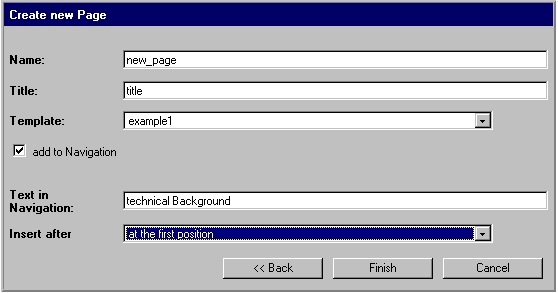
\includegraphics[clip,width=\sgw]{pics/modules/33}
\end{center}
\caption[Define the nav text]{Define the navigation text and the position 
when creating a new page.}
\label{NavText}
\end{figure}

The following example creates a simple navigation. The navigation class
scans the root directory for folders with meta-information for the
navigation. The folders and the files in these folders that contain
navigation meta-information are added to the navigation bar. This means
that the navigation includes two levels of the file tree: the folders
in the root directory and the files in these folders. Further
subdirectories are not included in the navigation.
To create a navigation you have to write your own template that
determines the layout for the navigation. In general, the look for the
selected entry of a navigation is different. You can define two
different data blocks for different looking navigation entries: one for
a selected entry and one for an entry that is not selected. Another
data block defines the layout for the headings in the navigation bar.
The headings are extracted from the navigation text of the folders in
the root directory. The values for the link target and link text are
defined in the Java class that builds the navigation. This class first
extracts the navigation information from the files and then inserts the
appropriate link in the document.\\

Here is the template that is used in this example:\\

\begin{xml}
<?xml version="1.0"?>\\
<xmltemplate>\\

<navhead>\\
<![CDATA[\\
<tr>\\
\xtaba <td nowrap colspan="2" >\\
\xtaba <a href="]]><process>navlink</process>\\
\xtaba <![CDATA[">]]><process>navtext</process><![CDATA[</a>\\
\xtaba </td>\\
</tr>\\
]]>\\
</navhead>\\
<navitem>\\
<![CDATA[\\
<tr>\\
\xtaba <td>\&\#8226;</td>\\
\xtaba <td nowrap>\\
\xtaba <a href="]]><process>navlink</process>\\
\xtaba <![CDATA[">]]><process>navtext</process><![CDATA[</a>\\
\xtaba </td>\\
</tr>\\
]]>\\
</navitem>\\
<navcurrent>\\
<![CDATA[\\
<tr>\\
\xtaba <td>\&gt;</td>\\
\xtaba <td nowrap>]]><process>navtext</process><![CDATA[</td>\\
</tr>\\
]]>\\
</navcurrent>\\
<navhome>\\
<![CDATA[\\
<p>\\
<table cellpadding="0" cellspacing="2" border="0">\\
<tr>\\
\xtaba <td nowrap colspan="2">\\
\xtaba <a href="]]><method name="getServletPath"/>\\
\xtaba <![CDATA[index.html">Homepage</a>\\
\xtaba </td>\\
</tr>\\
</table>\\
</p>\\
]]>\\
</navhome>\\
<template>\\
<![CDATA[\\
<p>\\
<table cellpadding="0" cellspacing="2" border="0">\\
]]>\\
<process>nav</process>\\
<![CDATA[\\
</table>\\
]]>\\
<process>navhome</process>\\
<![CDATA[\\
</p>\\
]]>\\
</template>\\
</xmltemplate>\\
\end{xml}

This template defines four data blocks for the different entries in the
navigation. The link and the text for the link are inserted via the
process tag. The data block {\name navhome} contains the link to the home
page and is statically defined in the template. The home page link
refers to the {\name index.html} file in the root directory.
Two data blocks are processed in the template: {\name nav} and {\name navhome.} The
data block {\name navhome} is the statically defined link to the home page.
The data block {\name nav} is defined  in the Java class and contains the
whole navigation bar.
The complete Java source code for the class that builds the navigation
will not be included in this document. Here, we will concentrate on
explaining the purpose of the program. Those of you who want to see the
full source code can take a look at the examples that are provided with
this document.

The program creates a vector of all of the subfolders of the root
folder by using the cms object:

Vector folders = {\name cms.getSubfolders("/");}

Three arrays are created that are big enough to hold as many entries as
are contained in the vector. One array is created for the navigation
links, one for the navigation texts, and one for the navigation

positions:
\begin{java}
int size = folders.getSize();\\
String navLink[] = new String[size];\\
String navText[] = new String[size];\\
float navPos[] = new float[size];\\
\end{java}

The next step is to extract the entries from the vector that should
appear in the navigation. Only those entries that have meta-information
about their navigation text and navigation position are included in the
navigation. The navigation entries are extracted and written to new
method called {\meth getNavEntries()}. This method returns an integer value
that contains the number of entries that will be included in the
navigation. The method takes the vector and the three arrays as
parameters and fills them with the different property entries:

{\code int max = getNavEntries(cms,folders,navLink,navText,navPos);}

The CmsObject is also passed to the method in order to obtain access to
the system resources. The CmsObject is used in the method {\meth getNavEntries()}
to extract the navigation meta-information as follows:

\begin{java}
CmsResource currentResource =\\
\jtabd     (CmsResource)resources.elementAt(i);\\
String path = currentResource.getAbsolutePath();\\
String pos = cms.readProperty(path, C\_PROPERTY\_NAVPOS);\\
String text = cms.readProperty(path, C\_PROPERTY\_NAVTEXT);\\
\end{java}

The {\class CmsResource} class is the base class for the CmsFolder class, which
is the type of the folders that are stored in the vector. First, the
path to the resource is extracted using the method {\meth getAbsolutePath()} of
the {\class CmsResource} class. The path is required to link to the document and
also to fetch the navigation properties by calling the {\meth readProperty()}
method of the CmsObject. The constants passed to the method are defined
in the interface  {\meth I\_CmsConstants}, which contains constants that are used
by the OpenCmsSystem. The constants {\meth C\_PROPERTY\_NAVPOS} and
{\meth C\_PROPERTY\_NAVTEXT} contain the string values {\code "NavText"} and {\code "NavPos."}

The next step is to check whether this navigation properties are
defined, i.e.  check whether the return value of {\meth getProperty()} is not
equal to the empty string or null. If the properties are defined, they
are stored in the arrays, which are sorted according to the navigation
positions. Sorting is implemented in a separate method. The used
algorithm is a selection sort, but it can be easily changed if necessary.
The entry for a folder is defined by setting the data blocks {\name navlink}
and {\name navtext} and appending the processed data block {\name navhead} to the
result:

\begin{java}
template.setData("navlink", servletPath + navLink[i] +\\
\jtabc    "index.html");\\
template.setData("navtext", navText[i]);\\
result.append(template.getProcessedDataValue("navhead"));\\
\end{java}

The steps performed for the folders are repeated for the files inside
the folders. This means that a check is performed to determine if they
should appear in the navigation. They are then sorted according to the
navigation positions. An entry for a file in a folder is either a
normal entry or the currently selected resource, which is displayed
differently:

\begin{java}
if (navLinkFile[j].equals(requestedUri)) \{\\
\jtabb  result.append(template.getProcessedDataValue("navcurrent"));\\
\} else \{\\
\jtabb  result.append(template.getProcessedDataValue("navitem"));\\
\}\\
\end{java}

This code checks whether the current file entry link (stored in the
array {\name navLinkFile[])} is equal to the requested resource. It then
appends the appropriate processed data block to the result. The data
block {\name "navcurrent"} is used for the currently selected navigation entry
and the data block {\name "navitem"} is used for the other entries.
The method then sets the data block {\name "nav,"} which contains the entire
navigation and starts the processing of the document:

\begin{java}
template.setData("nav", result.toString());\\
return startProcessing(cms, template, elementName, parameters,\\
templateSelector);\\
\end{java}

This navigation example creates a specific type of navigation, and is
used to provide insight into the methods and ways that are used to
create a navigation. The OpenCms system has a more elaborate and
generic navigation class that can be used to build more flexible and
sophisticated navigations. This class is the{\class  CmsXmlNav} class and can be
found in the {\name com.opencms.defaults} package. The information in this
section should help you to examine the way this class works and to use
its methods.

\subsection{Session management}
\index{session management}
Because the HTTP protocol is a stateless protocol there is usually no
way to recognize if consecutive requests are generated by the same
client. Each request is completely independent and has no influence or
memory of past or future requests. There is no built-in feature to keep
track of the user's actions in the HTTP protocol. OpenCms implements a
session management that enables user actions to be tracked. This
session management is built on the session tracking feature of the
original Servlet API . The user is recognized by placing a cookie on
the client side.  A cookie is  a little text file with a maximum amount
of 4096 bytes that is sent by the server and stored on the client. This
cookie contains a unique id string to identify a user. Session
management can also be used to store data. The session management layer
stores the class that is associated with a particular client in much
the same way a cookie is stored. Retrieving the class back again in a
subsequent request is a simple matter of calling a method from the
session management class.
Session management is essential when using the OpenCms workplace,
because OpenCms' entire user management relies on the session
management feature.

A session will be created or can be fetched by calling the {\meth getSession()}
method: {\meth CmsSession session =(CmsSession)cms.getRequestContext().getSession(true);}
\index{getRequestContext()}
\index{getSession}
If  the Boolean value is true and the session does not exist, a new
session is created. If the value false is passed with no session or
with an expired session, null is returned.
First, you have to get the CmsRequestContext object that contains the
access  to the related data. The specified parameter indicates that the
session will be created if it does not already exist. If you specify
false as the parameter value for the {\meth getSession()} method, it will
return null if a session did not previously exist. The returned object
is of the type {\class CmsSession} and can be used in a manner similar of that
of the original HTTP session objects of the Servlet API. However, only
some of the original methods provided by the Servlet API's HTTP Session
interface are provided by the {\class CmsSession} class. These methods are:

\begin{java}
public Object getValue(String name);\\
public void putValue(String name, Object value);\\
public void removeValue(String name);\\
\end{java}

As the name of the methods implies, they are used to fetch, store, or
delete session-related data. A session can be used much like a class
hash table when storing data in it. You can store every Java object
with a string as a key value to access the object.
It is {\bf important} to remove used and changed values before redirecting
them if they are no longer needed. You can easily archive them using
the above mentioned {\meth removeValue} method. Below is an example of how this
is done:

\begin{java}
if (session.getValue("myValue") != null)\\
        session.removeValue("myValue");\\
\end{java}

\subsubsection{A First Example Using Session Management}
The first example consists of two pages that show how to store data in
the session. In the first page, you can select different colors that
are represented by links with attached query strings. If you click on a
link, the attached query string is processed by the Java program, stored
in the session and displayed in the second page of the body template by
using the template selector mechanism. You can see the selected color
from the first page: it is used for the text and the background color.
Clicking on the link takes you back to the first page of the template.
Here, the color that you previously selected is displayed again.
The template consists of two pages that are alternately displayed. The
active template is selected by the template selector in the controlling
Java class:

\begin{java}
<?xml version="1.0"?>\\
<XMLTEMPLATE>\\
<TEMPLATE>\\
<![CDATA[\\
<body bgcolor="]]><PROCESS>bgcolor</PROCESS><![CDATA[">\\
<table width=70\% align=center valign=abscenter border>\\
<th><h1>Session Example</h1><br>\\
<h2>Select a color</h2>\\
<tr height=200 align=center><td><h2>Last color selected:<br>\\
]]><PROCESS>lastcolor</PROCESS><![CDATA[</h2>\\
</td></tr>\\
</table>\\
<table align=center valign=abscenter border=0>\\
<tr><td align=center><h2>\\
\jtabc        <a href="]]><METHOD\\
name="getServletPath"/><![CDATA[SessionBeispiel2.html?red">Red</a>\\
. . .\\
\jtabc        </h2></td>\\
</td></tr>\\
</table>\\
]]>\\
</TEMPLATE>\\
<TEMPLATE name="page2">\\
<![CDATA[\\
\jtabb     . . .\\
\jtabc        <h2>You just selected color:<br><h2></th>\\
\jtabc        <tr height=200 align=center ><td><h2>\\
\jtabc        ]]><PROCESS>bgcolor</PROCESS>\\
\jtabc        <![CDATA[</h2></td></tr>\\
\jtabb     . . .\\
\end{java}

This figure shows the default template output (the last color selected
was Blue) ... (figure~\ref{SessionExample}).

\begin{figure}
\begin{center}
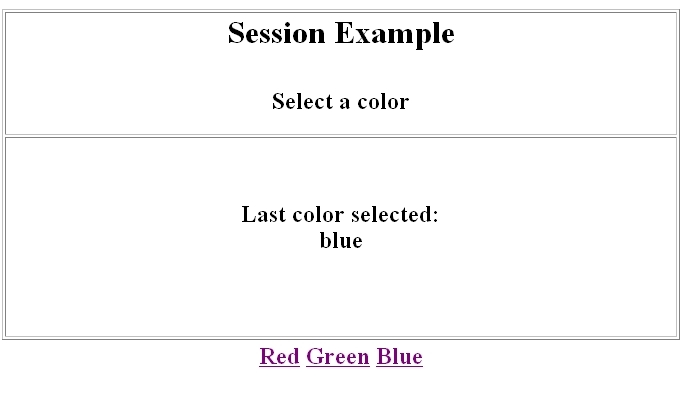
\includegraphics[clip,width=\sgw]{pics/modules/34}
\end{center}
\caption[Default template output Blue]{Default tmplate output Blue.}
\label{SessionExample}
\end{figure}

... and the template section named {\name "page2"} is activated by using the
templateSelector after clicking on a link (as you can see the color
Green was selected here) (figure~\ref{SessionExample2}).

\begin{figure}
\begin{center}
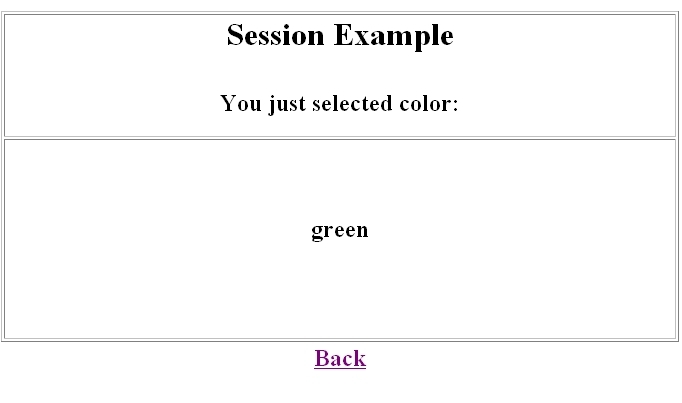
\includegraphics[clip,width=\sgw]{pics/modules/35}
\end{center}
\caption[Default template output Green]{Default template output Green.}
\label{SessionExample2}
\end{figure}

Here you can see the controlling Java method that stores the data in the
session and switches between the pages by setting the template selector.
In the session statement, a new session is created, or an existing one is
fetched. The color that was selected is attached to the HTTP request as
follows: http://www.opencms.org/sessionexample?colorvalue. To get the
query string that is attached to the HTTP link, the method
{\meth "getQueryString"} is called. If a color was saved in the previous session,
it is fetched again, and displayed on the first page as the last color
that was selected. On the first page, the user is able to select one of
three colors, whilst on the second page only the "back" link can be
selected. Depending on the link with the attached query string that is
selected by the user, the template selector is set to either the first
or the second page:

\begin{java}
public byte[] getContent(CmsObject cms, String templateFile, String\\
elementName, Hashtable parameters, String templateSelector) throws CmsException \{\\
\jtabc        //init\\
\jtabc        String colorValue;\\
\jtabc        String lastColorValue="";\\
CmsXmlTemplateFile templateDocument =\\
getOwnTemplateFile(cms, templateFile, elementName, parameters,\\
templateSelector);\\
//create new or fetch existing session\\
CmsSession session = (CmsSession)\\
cms.getRequestContext().getSession(true);\\
\jtabc        //get the query string from the link\\
colorValue = ""+((HttpServletRequest)\\
cms.getRequestContext().getRequest().\\
getOriginalRequest()).getQueryString();\\
\jtabc        //get the stored value from the session\\
\jtabc        lastColorValue = (String) session.getValue("colors2");\\
\jtabc        //go back to start page\\
\jtabc        if (colorValue == "back") \{\\
\jtabd                colorValue="null";\\
\jtabd                templateSelector="default";\\
\jtabb        \}\\
\jtabb        //color chosen?\\
\jtabb        if (colorValue !="null")\{\\
\jtabd                session.putValue("colors2",colorValue);\\
\jtabd                templateSelector="page2";//show second page\\
\jtabb        \}\\
\jtabb        //inital state of the page if (colorValue.equals("null") ||\\
colorValue.equals("") ||\\
colorValue.equals("back"))\{\\
\jtabe                        olorValue="white";\\
\jtabe                        emplateSelector="default";\\
\jtabb        \}\\
\jtabb        //set process data\\
\jtabb        templateDocument.setData("bgcolor",colorValue);\\
\jtabb        templateDocument.setData("lastcolor",lastColorValue);\\
return startProcessing(cms, templateDocument,\\
elementName, parameters, templateSelector);\\
\}\\
\}\\
\end{java}

\subsection {Session Content}
This example dumps the keys and corresponding values that are stored in
a session. The below example displays the preceding example's session
keys and values. As you can see, the value "red" attached to the clicked
link "Red" is stored in key "colors2" of the session. The other keys and
values were generated by the OpenCms system automatically for internal
use (figure~\ref{SessionExample3}).

\begin{figure}
\begin{center}
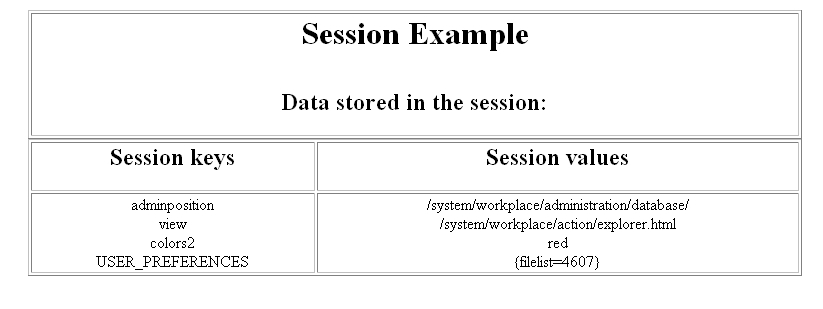
\includegraphics[clip,width=\sgw]{pics/modules/36}
\end{center}
\caption[Session Content Example]{Session Content Example.}
\label{SessionExample3}
\end{figure}

The keys of the fetched session are stored in a string array, and the
corresponding values are read out in a loop by the Java method. After
fetching the session, the session key strings are created by using the
{\meth "getValueNames"} method. By looping through the entries of this string
array the corresponding values are read out by the {\meth "getValues"} method.
Finally the data is set in the template document by using the {\name "setData"}
statement:

\begin{java}
public byte[] getContent(CmsObject cms, String templateFile,
String elementName, Hashtable parameters, String templateSelector)
throws CmsException \{\\
\jtabc        //init\\
\jtabc        String tempKey="";\\
\jtabc        String tempValue="";\\
CmsXmlTemplateFile templateDocument =\\
getOwnTemplateFile(cms, templateFile, elementName, parameters,\\
templateSelector);\\
\jtabc        //create new or fetch existing session\\
CmsSession session = (CmsSession)\\
cms.getRequestContext().getSession(true);\\
\jtabc        //copy sessionkeys into stringarray\\
String [] sessionKey = session.getValueNames();\\
\jtabc        //loop through sessionkeys\\
\jtabc        for(int i=0;i < sessionKey.length;i++) \{\\
\jtabd                tempKey += sessionKey[i]+"<br>";\\
tempValue += session.getValue(sessionKey[i])+"<br>";\\
\}\\
\jtabc        // set data in xml-document\\
\jtabc        templateDocument.setData("sessionkey", ""+tempKey);\\
templateDocument.setData("sessionvalue", ""+tempValue);\\
\jtabd                // Finally start the processing\\
\jtabc        return startProcessing(cms, templateDocument,\\
elementName, parameters, templateSelector);\\
\}\\
\end{java}

\subsection {Session history}
As mentioned above, you can store any object you like in the session,
e.g. strings, arrays or vectors. The following example makes use of this
feature by storing data of the past query strings in the session. The
example shows the past five color links you clicked and deletes the
oldest one, if you clicked more than five times (figure~\ref{SessionExample4}).

\begin{figure}
\begin{center}
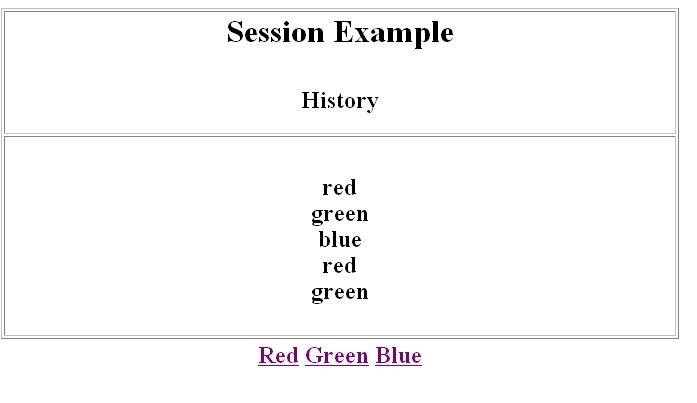
\includegraphics[clip,width=\sgw]{pics/modules/37}
\end{center}
\caption[Session history Example]{Session history Example}
\label{SessionExample4}
\end{figure}

This is done by the {\meth "getContent"} method described below. The values are
stored using a string array in the session. If the array is not empty,
it is fetched from the session. The new color value that is selected by
the user is appended to the first empty entry of the array. If there is
no empty entry left in the string array, the first entry is deleted by
shifting the other entries up by one position. The new entry is moved to
the (now empty) last position. The array is stored again in the session,
and the parameters for the template are processed.

\begin{java}
\jtabc        public byte[] getContent(CmsObject cms, String templateFile,\\
\jtabc        String elementName, Hashtable parameters, String templateSelector)\\
\jtabc         throws CmsException \{\\
\jtabc        //init\\
\jtabc        String allColorValues = "";\\
\jtabc        String colorValue="";\\
\jtabc        String[] colorArray= {"","","","","","",""} ;\\
\jtabc        //set data\\
\jtabc        CmsXmlTemplateFile templateDocument =\\
\jtabc        getOwnTemplateFile(cms, templateFile, elementName, parameters,\\
\jtabc        templateSelector);\\
\jtabc        //create new or fetch existing session\\
\jtabc        CmsSession session = (CmsSession)\\
\jtabc        cms.getRequestContext().getSession(true);\\
\jtabc        //get query string from link\\
\jtabc        colorValue =\\
\jtabc        ""+((HttpServletRequest)cms.getRequestContext()\\
\jtabc        .getRequest().getOriginalRequest()).getQueryString();\\
\jtabc        // get array data from the session\\
\jtabc        if (session.getValue("colorArray") !=null)colorArray = (String [])\\
\jtabc        session.getValue("colorArray");\\
\jtabc        // fill array with data\\
\jtabc        for (int i=0;i<6;i++)\{\\
\jtabd                if (colorArray[i] == "")\{\\
\jtabe                        colorArray[i]=colorValue;\\
\jtabe                        break;\\
\jtabd                \}\\
\jtabc        \}\\
\jtabc        // if array filled shift array data\\
\jtabc        if (colorArray[5] != "") \{\\
\jtabd                for(int i=0;i<6;i++)\{\\
\jtabe                        colorArray[i]=colorArray[i+1];\\
\jtabd                \}\\
\jtabd                colorArray[5]="";\\
\jtabc        \}\\
\jtabc        for (int i=0;i<6;i++) allColorValues += "<br>"+colorArray[i];\\
\jtabc        //store data in the session session.putValue("colorArray",colorArray);\\
\jtabd                session.putValue("colors",colorValue);\\
\jtabc        //set parameters for processing\\
\jtabc        if (colorValue.equals("null") ||colorValue.equals("")) colorValue="white";\\
\jtabc        templateDocument.setData("bgcolor",colorValue)
\jtabc        ;templateDocument.setData("button",allColorValues);\\
\jtabc        return startProcessing(cms, templateDocument, elementName,
\jtabc        parameters, templateSelector);\\
\jtabc        \}\\
\}\\
\end{java}

Session management is a useful feature when building web sites with
OpenCms because it enables you to implement advanced features such as
HTML forms that extend over multiple pages, online shopping functionality
or personalized web content. Session management extends the abilities of
cookies that are only capable of storing text data of a limited size
(4096 Bytes) on the client. With session management, it is possible to
store binary and class information. The session management is, of course,
not only usable with query strings but also with forms. The next chapter
explains how forms are used with the template mechanism.

\section{Forms}
HTML forms are used to add functionality to a web site. With HTML forms,
you can receive feedback from the surfers or enable them to order
products, product-related materials, or anything else you'd like to make
available.
The input that is received from the user can be evaluated in a number of
ways. Traditionally, this is done by a cgi program that processes the
data on the server. Major drawbacks of this approach are the
inefficiency and the security holes. When using cgi programs to process
the data, every request to the cgi program creates a new process, which
produces a significant load on the operating system. The cgi approach
does not come with a security model that prevents incorrect cgi programs
from crashing the server.
These disadvantages have been overcome by Java servlets, which provide a
way to write efficient, platform independent, and secure
server-applications. Servlets are special Java classes that can be
executed by a server that supports the Java servlet API. Servlets take
advantage of the built in security model and the platform independence
of the Java language. An instance of a servlet is loaded either when the
server is started (this can be specified by in the server's Services) or
when the servlet is first accessed. Concurrent requests to one servlet
are handled by multiple threads of the servlet. After a servlet is first
loaded and initialized, it is generally not unloaded until the server
shuts down. This ensures the servlet class is loaded and initialized
once when the servlet is accessed for the first time.
OpenCms itself is a servlet that enables the evaluation of HTML forms
writing customized Java classes. Although not servlets themselves, these
classes have the same advantages as servlets: they are efficient,
portable, and secure!
This chapter explains how input fields, radio buttons or select buttons
are used in forms. It also discusses programming techniques that can
(and should) be used with forms, such as validating and error checking
input, as well as re-displaying input in input fields. Starting with the
simple re-display of text that was typed in an input field, you will
learn how to use radio buttons and evaluate input data for errors
(empty fields or incorrect inputs).

\subsection {A first example using forms}
In a first and simple example, you will see how a form can be used for
plain text input and re-to re-display the output on a confirmation page
after pressing a button.

Because the form shouldn't be evaluated when it is requested for the
first time, a little trick can help to detect if the page is being
displayed for the first time or if it has already been filled out. A
hidden input field in the form acts as a flag that indicates if the
input fields have to be checked or not. A hidden input field works
similar to a cookie, except that cookies are sent for every request and
not just in response to a form posting. The value of this hidden field
is set in the Java class. When the page is first requested, the value of
the field is not defined. The Java class detects this and omits checking
the input fields. This is the section with the hidden input field:

\begin{java}
<FORM>...\\
<INPUT type="hidden" name="action"\\
value="]]><process>setaction</process><![CDATA[">\\
...</FORM>\\
The Java class reads in the parameter and does something like this:\\
...\\
String action = (String) parameters.get("action");\\
//no button pressed!\\
if (action == null || action.equals("")) \{\\
\jtabc        templateSelector="default";\\
\jtabc        template.setData("setaction","default");\\
...\\
\end{java}

This is the first page of the template with some content. It consists of
two different input fields in which free text can be entered (figure~\ref{FreeText}).

\begin{figure}
\begin{center}
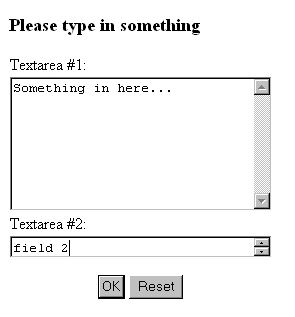
\includegraphics[clip,width=0.4\linewidth]{pics/modules/38}
\end{center}
\caption[Template with some content.]{Template with some content.}
\label{FreeText}
\end{figure}

After typing in the text, you can click on the OK or the Reset button.
These two are the standard buttons that are used with HTML forms.
Clicking on one of these buttons sends the form data.

\begin{java}
<INPUT type=submit value="OK">\\
<INPUT type=reset value="Reset">\\
\end{java}

The Reset button automatically erases the input field without sending
the data. Clicking on the OK button displays the text in the input
fields on the second page of the template. The form tag determines the
method that is used to send the data to the server. The controlling Java
class selects the appropriate template by setting the template selector
with the name of the template section.
This is the result on the confirmation page after clicking on the OK
button (figure~\ref{TypeIn}).

\begin{figure}
\begin{center}
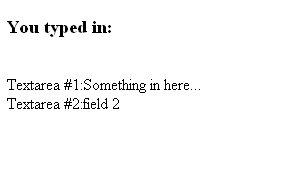
\includegraphics[clip,width=0.5\linewidth]{pics/modules/39}
\end{center}
\caption[Results on the confirmation page]{Results on the confirmation page.}
\label{TypeIn}
\end{figure}

As you can see, the confirmation page shows the user his/her input again
so that he/she can see what was sent to the server. The confirmation
page is selected in the Java class by setting the template selector.
Assuming you have named the confirmation template {\name "reply,"} all you have
to do to tell OpenCms that this template should be used to create the
web page that is shown to the user, is to set the template selector in
your class:

{\code .. templateSelector="reply"; ...}

After storing the information in the session, the data is fetched from
the session again when the confirmation page "reply" is selected by the
template selector:

\begin{java}
public byte[] getContent(CmsObject cms, String\\
templateFile, String elementName, Hashtable parameters, String
templateSelector) throws CmsException \{\\
//init\\
\jtabc        CmsXmlTemplateFile templateDocument =getOwnTemplateFile(cms, templateFile,\\
 elementName, parameters,templateSelector);\\
\jtabc        //create new or fetch existing session\\
\jtabc        CmsSession session = (CmsSession)cms.getRequestContext().getSession(true);\\
\jtabc        //get the stored value from the session\\
\jtabc        String comment = (String) session.getValue("comment");\\
\jtabc        String comment2 = (String) session.getValue("comment2");\\
//button pressed? String action = (String) parameters.get("action");\\
\jtabc        //no button pressed!\\
\jtabc        if (action == null || action.equals("")) \{\\
\jtabe                templateSelector="default";\\
\jtabe                templateDocument.setData("setaction","default");\\
\jtabc        //a button was pressed\\
\jtabc        \} else \{\\
\jtabd              //get parameters from the default template\\
\jtabd              comment = ((String) parameters.get("comment"));\\
\jtabd              comment2 = ((String) parameters.get("comment2"));\\
\jtabd              //set the template selector\\
\jtabd                templateSelector="reply";\\
\jtabd                //set the parameters in the reply template\\
\jtabd                templateDocument.setData("setaction","reply");\\
\jtabd                templateDocument.setData("comment",comment);\\
\jtabf                templateDocument.setData("comment2",comment2);\\
\}\\
return startProcessing(cms, templateDocument,\\
\jtabd      elementName, parameters, templateSelector);\\
\}\\
\end{java}


\subsection {Presetting values}
In order to use preset values, the controlling Java class has to set the
values of the fields with a preset value or with the input the user has
already given. This can be accomplished by setting the value of a field
via the process tag:

\begin{java}
<TEXTAREA cols=30 rows=8 name=comment>\\
]]><process>comment</process><![CDATA[\\
</TEXTAREA>\\
\end{java}

The value of the input field will be the value of the data block comment.
This data block is specified in the template as an empty data block: If
you did not initialize the data block, you will get an error message
that the data block is unknown. You should always define the value  as
an empty element in the beginning of the body template:

\begin{xml}
<XMLTEMPLATE>...\\
<comment></comment> ...\\
<TEMPLATE>...\\
\end{xml}

A value is preset by entering text. When the template is first started,
the data block is set with this value:

\begin{xml}
<XMLTEMPLATE>...\\
<comment>Please fill in something here!</comment>...\\
<TEMPLATE>...\\
\end{xml}

If the value is not defined in the Java class with a different value,
the data block will be empty or set to the start value, if it was
defined in the template. To show the user's input in the field, the
input first has to be fetched from the parameters that were passed to
the getContent() method, which will set the data block comment to this
value. Below is a piece of code that shows how to do this:

\begin{xml}
String comment = (String) parameters.get("comment");\\
template.setData("comment", comment);\\
\end{xml}

The value of the field is first fetched from the parameters' hash table,
which stores the parameters that are passed when the form is submitted.
The data block is then set to this value. When started for the first
time, the output of the example page with the preset comment data block
"Please fill in something here!" would look like this (figure~\ref{TypeIn1}).

\begin{figure}
\begin{center}
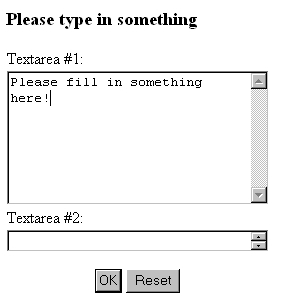
\includegraphics[clip,width=0.5\linewidth]{pics/modules/40}
\end{center}
\caption[Presetting values pic1]{Presetting values Pic 1.}
\label{TypeIn1}
\end{figure}

\subsection {Evaluating forms}
It is desirable to evaluate input fields for empty or invalid data and
to give feedback to the user if input fields were filled out incorrectly.
Form evaluation is a typical task that is performed by a programmer.
The error checking and validation processes have to be provided by the
controlling Java class. In the following example, the user is asked to
fill out the input fields with his name, e-mail address and telephone
number. The fields marked with an * are required, the telephone number
is optional (figure~\ref{EvaluForms}).

\begin{figure}
\begin{center}
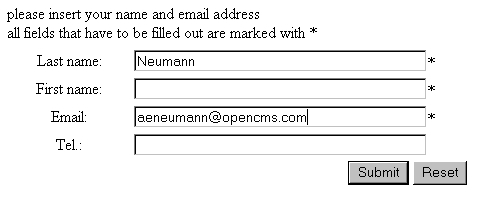
\includegraphics[clip,width=0.7\linewidth]{pics/modules/41}
\end{center}
\caption[Evaluating forms Pic 1]{Evaluating forms Pic 1.}
\label{EvaluForms}
\end{figure}

After posting the form data to the server by clicking on the OK button,
the input fields are checked by the Java class, to see if any of the
required (*) fields were left empty. The page is re-displayed with the
data that the user typed in and error messages. The user is informed
that  some of the fields were not correctly filled out. In the above
example, the user forgot to fill out the First Name input field. The
follow message is displayed and access to the confirmation page denied
(figure~\ref{EvaluForms1}).

\begin{figure}
\begin{center}
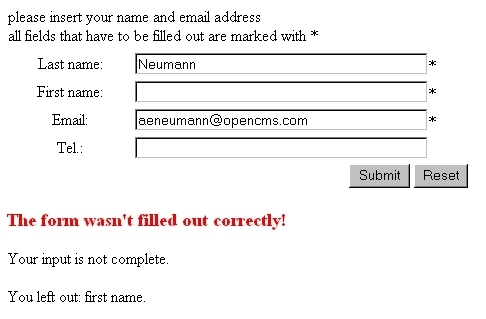
\includegraphics[clip,width=0.7\linewidth]{pics/modules/42}
\end{center}
\caption[Evaluating forms Pic 2]{Evaluating forms Pic 2.}
\label{EvaluForms1}
\end{figure}

The Java class uses preset data blocks with text phrases in the template
to display the error message in the error process at the end of the form
tag. If the input is correct, the error data block remains empty (as
initialized in the template). If there are errors (one or more of the
first three fields are empty) the page is re-displayed with the error
message using the text in the {\name init} section:
\index{error message}
\begin{java}
...\\
<!--init-->\\
<FIELD\_OMITTED><![CDATA[Your input is not complete.<br></br>\\
You left out: ]]>\\
</FIELD\_OMITTED>\\
<MISSING\_LAST\_NAME><![CDATA[last name]]></MISSING\_LAST\_NAME>\\
<MISSING\_FIRST\_NAME>\\
<![CDATA[first name]]>\\
</MISSING\_FIRST\_NAME>\\
<MISSING\_EMAIL><![CDATA[e-mail]]></MISSING\_EMAIL>\\
<GENERAL\_ERROR>\\
<![CDATA[<font color=\#FF0000><h3>The form wasn't filled out correctly!\\
</h3></font>]]>\\
</GENERAL\_ERROR>\\

<KOMMA><![CDATA[, ]]></KOMMA>\\
<POINT>.</POINT>\\
<BREAK><![CDATA[<br></br>]]></BREAK>\\
<NO\_VALUE><![CDATA[none]]></NO\_VALUE>\\

<setaction></setaction>\\
<first\_name></first\_name>\\
<last\_name></last\_name>\\
<tel></tel>\\
<email></email>\\
<error></error>\\
<!--end init-->\\
...\\
<FORM method="post">\\
...\\
<INPUT type=text maxLength=40 name=last\_name\\
value="]]><process>last\_name</process>\\
<![CDATA[" size=40>*\\
...\\
<INPUT type="hidden" name="action" value="default">\\
</FORM>\\
]]><process>\bf{error}</process><![CDATA[...\\
\end{java}


After the form data is sent, the Java code fetches the data from the
hash table. It then checks the data for missing input by looking for
empty strings. If empty fields are found, an error message is generated,
and the missing data field names are concatenated with data blocks that
contain text from the template to create a more readable output of the
error message. If one field is left empty, the integer fields are
incremented and the Boolean value of the error is set to true. The
missing fields are concatenated using the data block text contained in
the template. Last but not least, the error text is returned. Below you
can see the code of the Java methods that provide the evaluation of the
input fields:

\begin{java}
private StringBuffer checkInput(Hashtable parameters,CmsXmlTemplateFile template)throws CmsException \{\\
\jtabc        boolean error = false;\\
\jtabc        boolean emailError = false;\\
\jtabc        StringBuffer errorText = new StringBuffer();\\
\jtabc        String[] missingFields = new String[3];\\
\jtabc        int fields = 0;\\
\jtabc        String lastName = ((String) parameters.get("last\_name"));\\
\jtabc        String firstName = ((String) parameters.get("first\_name"));\\
\jtabc        String email = ((String) parameters.get("email"));\\
\jtabc        String tel = ((String) parameters.get("tel"));\\
\jtabc        // check if the fields last\_name, first\_name\\
\jtabd         // and email are filled out\\
\jtabc        if {\bf(lastName.equals(""))}\\
\jtabe                missingFields[fields++] = "missing\_last\_name";\\
\jtabc        if {\bf(firstName.equals(""))}\\
\jtabe                missingFields[fields++] = "missing\_first\_name";\\
\jtabe        if {\bf(email.equals("")}) missingFields[fields++] =\\
\jtabf         "missing\_email";\\
\jtabe        // create error message when fields are omitted\\
\jtabe        if (fields > 0) \{\\
\jtabf                error = true;\\
\jtabf                errorText.append(template.getDataValue("field\_omitted"));\\
\jtabf                for (int i = 0; i < fields; i++) \{\\
\jtabf                        errorText.append(template.getDataValue(missingFields[i]));\\
\jtabf                        if (i < fields - 1) \{\\
\jtabf                        errorText.append(template.getDataValue("komma"));\\
\jtabf                        \}\\
\jtabf                \}\\
\jtabf                errorText.append(template.getDataValue("point"));\\
\jtabf                errorText.append(template.getDataValue("break"));\\
\jtabe        \}\\
\jtabe        if (error) \{\\
\jtabf        errorText.insert(0,template.getDataValue("general\_error"));\\
\jtabf                if (emailError) \{\\
\jtabe        errorText.append(template.getDataValue("email\_error"));\\
\jtabf                \}\\
\jtabe        \}\\
\jtabe        return errorText;\\
\}\\
\end{java}

The method {\meth "getContent"} calls the above seen "checkInput" method, which
returns the error message. The rest of the coding is more or less the
same as seen in the previous examples:

\begin{java}
...\\
\jtabc        //no button pressed!\\
\jtabc        if (action == null || action.equals("")) \{\\
\jtabd                templateSelector="default";\\
\jtabd                template.setData("setaction","default");\\
\jtabc        //the ok button was pressed\\
\jtabc        \} else \{\\
\jtabd                String errorText="";\\
\jtabd                //check input for errors\\
\jtabd                errorText = checkInput(parameters,template).toString();\\
\jtabd                String lastName = ((String)parameters.get("last\_name"));\\
\jtabd                String firstName = ((String)parameters.get("first\_name"));\\
\jtabd                String email = ((String) parameters.get("email"));\\
\jtabd                String tel = ((String) parameters.get("tel"));\\
\jtabd                // set the fields with the given input in any case \\
\jtabd            // (even if empty String)\\
\jtabd                template.setData("last\_name", lastName);\\
\jtabd                template.setData("first\_name", firstName);\\
\jtabd                template.setData("email", email);\\
\jtabd                template.setData("tel", tel);\\
\jtabd                // if no error show reply template\\
\jtabd                if (errorText.length() == 0) \{\\
\jtabf                                templateSelector = "reply";\\
\jtabd                \} else \{\\
\jtabe                        // show default page again with error message\\
\jtabe                        templateSelector = "default";\\
\jtabe                        // set error text \\
\jtabe                        template.setData("error", ""+errorText);\\
\jtabd                \}\\
\jtabc        \}\\
\jtabc        return startProcessing(cms, template, elementName,parameters, templateSelector);\\
\}\\
\end{java}

\subsection{Validating Forms}
In order to perform a detailed check of the input data, the text must be
checked for invalid content. The above example is extended by a simple
e-mail checker. The Java method considers the e-mail address to be
valid  if it consists of at least one character before the @ sign, the @
sign itself, one more character, a dot (.) and at least two more
characters, but three at the most, that represent the domain. If this is
not the case, the user gets the following error message
(figure~\ref{ValidaForms}).

\begin{figure}
\begin{center}
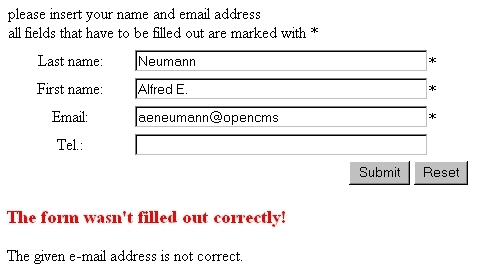
\includegraphics[clip,width=0.7\linewidth]{pics/modules/43}
\end{center}
\caption[Validating forms Pic 1]{Validating forms Pic 1.}
\label{ValidaForms}
\end{figure}

To validate the e-mail address, the Java method {\meth checkInput} is simply
extended in the mail checking section by calling the {\meth validEmail} method:

\begin{java}
...\\
if (email.equals("")) \{\\
\jtabc        missingFields[fields++] = "missing\_email";\\
\jtabc       \} else \{\\
\jtabc        if (!validEmail(email)) \{\\
\jtabe                error = true;\\
\jtabe                emailError = true;\\
\jtabc        \}
\}\\
...\\
\end{java}

The method {\meth validEmail} returns true if a check is performed and the
e-mail address is valid, and false in all remaining cases. This method
performs an extended check of the e-mail address. First, the unnecessary
spaces are removed by the trim method. Then the e-mail address is
checked for correctness by running through the string:

\begin{java}
\index{validEmail}
private boolean validEmail(String email) \{\\
\jtabc        email = email.trim();\\
\jtabc        String name = null;\\
\jtabc        String server = null;\\
\jtabc        boolean retVal = false;\\
\jtabc        int indexOfAt = -1;\\
\jtabc        int indexOfPoint = -1;\\
\jtabc        int length = email.length();\\
\jtabc        for (int i = 0; i < length; i++) \{\\
\jtabe                if (email.charAt(i) == '@') \{\\
\jtabf                        if (indexOfAt == -1) \{\\
\jtabf                                indexOfAt = i;\\
\jtabf                        \} else \{\\
\jtabf                        // more than one @ in the address !!!\\
\jtabf                        return false;\\
\jtabf                        \}\\
\jtabe                \}\\
\jtabc        \}\\
\jtabc        if (indexOfAt > 0 \&\& indexOfAt < length - 4) \{\\
\jtabe                name = email.substring(0, indexOfAt);\\
\jtabe                server = email.substring(indexOfAt);\\
\jtabe                length = name.length();\\
\jtabe                // first and last character of the name should not be a dot\\
\jtabe                if ((name.charAt(0) != '.')\\
\jtabf                        \&\& (name.charAt(length - 1) != '.')) \{\\
\jtabf                        // check if there are two consecutive dots in the name\\
\jtabf                        for (int i = 1; i < length - 1; i++) \{\\
\jtabf                                if (name.charAt(i) == '.') \{\\
\jtabf                                        if (indexOfPoint < i - 1) \{\\
\jtabf                                                indexOfPoint = i;\\
\jtabf                                        \} else \{\\
\jtabf                        // there are two consecutive dots (..)\\
\jtabf                                                return false;\\
\jtabf                                        \}\\
\jtabf                                \}\\
\jtabf                        \}\\
\jtabf                        length = server.length();\\
\jtabf                        // first character not a dot '.'\\ 
\jtabf                    // and at least two characters after last dot\\
\jtabf                        if ((server.charAt(0) != '.')\\
\jtabf                \&\& server.lastIndexOf('.') < length - 2) \{\\
\jtabf                                indexOfPoint = -1;\\
\jtabf                                for (int i = 1; i < length - 2; i++) \{\\
\jtabf                                        if (server.charAt(i) == '.') \{\\
\jtabf                                                if (indexOfPoint < i - 1) \{ \\
\jtabf                                                    indexOfPoint = i;\\
\jtabf                                                \} else \{\\
\jtabf                                // there are two consecutive dots (..)\\
\jtabf                                                        return false;\\
\jtabf                                                \}\\
\jtabf                                        \}\\
\jtabe                                \}\\
\jtabf                  // at least one '.' in server name and no more than\\
\jtabf                  // three characters after the last dot\\
\jtabe                                if ((indexOfPoint != -1)\\
\jtabe                    \&\& (indexOfPoint >= length - 4)) \{\\
\jtabf                                        retVal = true;\\
\jtabe                                \}\\
\jtabd                        \}\\
\jtabc                \}\\
\jtabb        \}\\
return retVal;\\
\}\\
\end{java}

\subsection{Using Radio Buttons and Check Boxes}
HTML provides check boxes and radio buttons for limited selections.
Radio buttons enable users to specify a selection by clicking on a field
rather than by inputting data. Check boxes represent a group of labeled
buttons in HTML. The user is able to check none, one or more of these
buttons that belong to the same group, which is defined by the name of
the value. The check box is defined in HTML as an input field tag with
the type check box. Check boxes are defined in HTML forms by the
following syntax:

\begin{java}
<input  type=checkbox name="my\_name" value="some\_value">
checkbox\_description
\end{java}
\index{checkbox}

Radio buttons are very similar to check boxes, except for the fact that
the user has to check exactly one button of the same group. The group is
defined by the name of the value. Clicking on another radio button
switches the old selection to the new one. The defined value is sent by
the form when the data is confirmed by clicking on the OK button. Radio
buttons are defined in HTML forms by:

\begin{java}
<input type=radio name="my\_name" value="some\_value">\\
radiobutton\_description\\
\end{java}
\index{radio}

Below is an example of a form that used both radio buttons and check
boxes. The user's selection consists of one of four radio buttons within
one group, and of three check boxes within another group 
(figure~\ref{Feedback}).

\begin{figure}[t]

\begin{minipage}[b]{0.49\linewidth}
\begin{center}
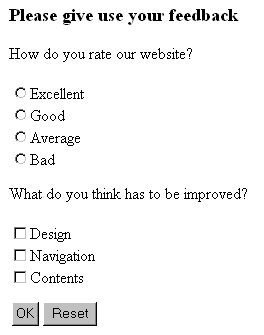
\includegraphics[clip,width=0.5\linewidth]{pics/modules/44}
\end{center}
\end{minipage}
\hfill
\begin{minipage}[b]{0.49\linewidth}
\begin{center}
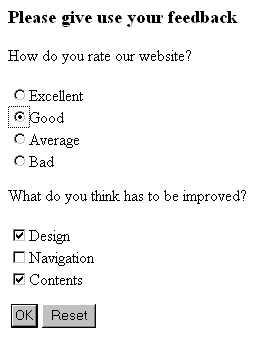
\includegraphics[clip,width=0.5\linewidth]{pics/modules/45}
\end{center}
\end{minipage}

\caption[Usage of Radio buttons]{Usage of Radio buttons}
\label{Feedback}

\end{figure}

The radio button{\name Good} and the check boxes {\name Design} and {\name Contents} were
clicked by the user before the confirmation button was activated (figure~\ref{Feedback}).
The Java method {\meth checkRadio} is used to test, if a radio button was
checked and then return the value {\name checked}. The Java method  is called
by a method tag with two parameters name and value in the body template.
The method returns {\name checked}, if  a radio button was pressed. This is
the section in the template containing the input fields calling the
method {\meth checkRadio}:

\begin{java}
...\\
<INPUT type=checkbox name=design value="design"]]>\\
<method name="checkRadio">design,design\\
</method><![CDATA[>Design\\
<INPUT type=checkbox name=nav value="navigation"]]>\\
<method name="checkRadio">nav,navigation\\
</method><![CDATA[>Navigation\\
<INPUT type=checkbox name=cont value="contents"]]>\\
<method name="checkRadio">cont,contents\\
</method><![CDATA[>Contents\\
...\\
\end{java}

If something was checked in the selection, the {\meth checkRadio} method
inserts the value {\name checked} to the template for both radiobuttons and
checkboxes. Everything that was selected in the body template, is stored
in the session hash table for further processing after pressing the OK
button. So you just have to fetch the data of the session again in the
{\meth getContent} method for further processing:

\begin{java}
public Object checkRadio(CmsObject cms, String tagcontent,\\
A\_CmsXmlContent doc, Object userObject)throws CmsException \{\\
\jtaba        Hashtable parameters = (Hashtable) userObject;\\
\jtaba        String returnValue = "";\\
\jtaba        int kommaIndex = tagcontent.indexOf(",");\\
\jtaba        if (kommaIndex > 0) \{String radioGroup = tagcontent.substring(0,kommaIndex);\\
\jtabb                String radioName = tagcontent.substring(kommaIndex + 1);\\
\jtabb                String selected = (String) parameters.get(radioGroup);\\
\jtabb                if (selected != null \&\& selected.equals(radioName)) \{\\
\jtabc                        returnValue = "checked";\\
\jtabb                \}\\
\jtaba        \}\\
\jtaba        return returnValue;\\
\}\\
\end{java}

The {\meth "getContent"} method processes the checked boxes by getting them from
the session's hash table and displaying the result on the confirmation
page (the template section  {\name "reply")} of the template. Pre-defined data
blocks in the body template that contain text are used to process a
readable error message:

\begin{java}
...\\
//a button was pressed\\
\} else \{\\
// get value of radio button group rating\\
// possible values: excellent, good, average, bad\\
\jtaba        String rating = (String) parameters.get("rating");\\
\jtaba        // if no rating was selected put error message on screen\\
\jtaba        if (rating == null || rating.equals("")) \{\\
\jtabb                errorText.append(template.getDataValue("rating\_error"));\\
\jtabb                template.setData("error", errorText.toString());\\
\jtabb                // set hidden field action to value "reply"\\
\jtabb                template.setData("setaction", "reply");\\
\jtaba        \} else \{\\
\jtabb                // get values of checkboxes design, nav and cont\\
\jtabb                String design = (String) parameters.get("design");\\
\jtabb                String nav = (String) parameters.get("nav");\\
\jtabb                String cont = (String) parameters.get("cont");\\
\jtabb                // show next page\\
\jtabb                templateSelector = "reply";\\
\jtabb                String[] improveWhat = new String[3];\\
\jtabb                int count = 0;\\
\jtabb                StringBuffer improveText = new StringBuffer();\\
\jtabb                // create the sentence about what should be improved\\
\jtabb                // check which checkboxes have been selected\\
\jtabb                if (design != null) improveWhat[count++] = "design";\\
\jtabb                if (nav != null) improveWhat[count++] = "navigation";\\
\jtabc                        // create a list for more than one entry\\
\jtabc                        if (count > 1) \{\\
\jtabd                           improveText.append(\\
\jtabf                  template.getDataValue("improve\_list\_begin"));\\
\jtabd                           for (int j = 0; j < count; j++) \{\\
\jtabd                             template.setData("item",\\ 
\jtabf                  template.getDataValue(improveWhat[j]));\\
\jtabe                             improveText.append(\\
\jtabf                  template.getProcessedDataValue("list\_item"));\\
\jtabd                          \}\\
\jtabd                improveText.append(template.getDataValue("improve\_list\_end"));\\
\jtabc                        \}\\
\jtabc                        // create a sentence if only one entry\\
\jtabc                        if (count == 1) \{\\
\jtabd              template.setData("improve\_only\_what",\\
\jtabd              template.getDataValue(improveWhat[0]));\\
\jtabd              improveText.append(template.getProcessedDataValue("improve\_only"));\\
\jtabc                        \}\\
\jtabc                        template.setData("rating", rating);\\
\jtabc                        template.setData("improvement", improveText.toString());\\
\jtabb                \}\\
\jtaba        \}\\
\jtaba        return startProcessing (cms, template, elementName, parameters, templateSelector);\\
\}\\
\end{java}

This is the message that the {\meth "getContent"} method produces if the input
is complete (a radio button and one or more check boxes were checked)
(figure~\ref{Feedback3}).

\begin{figure}
\begin{center}
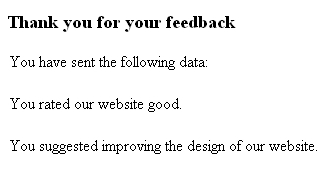
\includegraphics[clip,width=0.6\linewidth]{pics/modules/46}
\end{center}
\caption[Radio buttons Pic 3]{Radio buttons Pic 3.}
\label{Feedback3}
\end{figure}

\subsection {Presetting the Values of Select Boxes and Radio Buttons in Java}
As we have seen in the previous examples, presetting the values of radio
buttons is a bit tricky. OpenCms takes care of this problem by providing
a special template class called CmsXmlFormTemplate that facilitates the
control of select boxes and radio buttons from within the controlling
Java class. This template class allows radio buttons and select boxes to
be selected before the body template is started. If you want to create
radio buttons or select boxes with Java, your Java class has to extend
the CmsXmlFormTemplate rather than the normally used template class
CmsXmlTemplate.

The standard HTML input tag select box that is used in the body template
has to be replaced by the following method tag, which is structured in
much the same way the original HTML tag is. In its plainest form the tag
looks like this:

{\code ]]><select name="select\_1" method="my\_selectorMethod"/><![CDATA[}

The standard radio button input field is replaced by the following
method tag:

{\code ]]><radio name="radio\_1" method="my\_selectorMethod" order="row"/><![CDATA[}

The main difference between the two basic tags shown above is that you
can display the radio buttons in a row or in a column layout.

The layout of the radio buttons and select boxes is defined in a special
file. Without this file, the new radio and select tags will not work.
You need to extend your workplace by the HTMLFormDefs file in the
/content/internal directory because this file is used by the methods
{\tag handleRadiobuttonTag} and {\tag handleSelectTag} of the {\class CmsXmlFormTemplate
class.}

If you want to use additional statements in these tags (e.g. to change
the size) have a look at the HTMLFormDef file that can be found in your
{\dir content/internal/} directory.

Below is an example with the values "elite" for the radio button and
"other" for the select box set by the Java method (figure~\ref{RadioButtons}).

\begin{figure}
\begin{center}
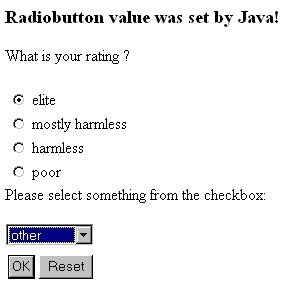
\includegraphics[clip,width=0.4\linewidth]{pics/modules/47}
\end{center}
\caption[Radio buttons in Java]{Radio buttons in Java.}
\label{RadioButtons}
\end{figure}

You can activate the radio button that should be pre-selected by setting
the data  in the session by a method in your Java class (normally the
{\meth "getContent"} method). In this example, the Java code session.putValue
{\meth("checkradio", "my\_radioname\_1")}activates the radio button
{\meth "my\_radioname\_1."}

The layout is set with {\name "order="} to rows or columns.

The template calls the method{\meth "my\_radioMethod"} in the radio element.
The checked radio button that was stored in the session is displayed
with the other names and values that were added to this method.

\begin{java}
public Integer my\_radioMethod (CmsObject cms, Vector values, Vector names, Hashtable parameters)\\
\jtabb                  throws CmsException \{\\
\jtabb                  int index;\\
\jtaba                String checkradioValue = (String)session.getValue("radio\_1");\\
\jtaba                // add values for the checkbox\\
\jtabb                   values.addElement("my\_radiovalue\_1");\\
\jtaba                ...\\
\jtaba                // add corresponding names for the checkboxvalues\\
\jtabb                   names.addElement("my\_radioname\_1");\\
\jtaba                ...\\
\jtaba                // used for the assignment of the button\\
\jtabb                   if checkradioValue.equals("my\_radiovalue\_1")\\
\jtaba                index = 0;\\
\jtaba                ...\\
\jtaba                return new Integer(index);\\
                \}\\
\end{java}

To set the initial value (e.g. in the {\meth "getContent"} method or even in
the {\meth "my\_radio\_method"} itself), you have to create a new session (fetch
an existing one) and store the value that is to be displayed when the
body template is first started in the session:  (here: {\meth "my\_radiovalue\_1")}:

\begin{java}
...\\     
CmsSession session = (CmsSession)\\
cms.getRequestContext().getSession(true);\\
...\\     
session.putValue("radio\_1","my\_radiovalue\_1");\\
\end{java}

You can activate the select box entry that should be initially displayed
by setting the data to activate the select box item {\name (to "my\_name")} in
the session by a method in your Java class (normally the {\meth "getContent"}
method). Your Java code should look like this:

{\code session.putValue("checkselect","my\_selectname\_1".}

The template calls the method {\meth "my\_selectorMethod"} in the select element
tag. The selected select box item that was stored in the session is
displayed. The other select box names become visible after select box
is opened.

\begin{java}
public Integer my\_selectorMethod (CmsObject cms, Vector values, Vector names, Hashtable parameters)\\
\jtabb                throws CmsException \{\\
\jtabb                int index;\\
\jtaba          String checkselectValue = (String)\\
\jtaba        session.getValue("selectbox\_1");\\
\jtaba        // add values for the selectbox\\
\jtaba        values.addElement("my\_selectvalue\_1");\\
\jtaba        ...\\
\jtaba        // add corresponding names for the selectboxvalues\\
\jtaba        names.addElement("my\_selectname\_1");\\
\jtaba        ...\\
\jtaba        // used for the assignment of the button\\
\jtaba        if checkselectValue.equals("my\_selectvalue\_1") index = 0;\\
\jtaba        ...\\
\jtaba        return new Integer(index);\\
\}\\
\end{java}

To set the initial value (e.g. in the {\meth getContent} method or even in the
{\meth my\_selector\_method} itself), you have to create a new session (fetch an
existing one) and store the value that is to be displayed when the
template is first started in the session: (here: {\meth my\_selectvalue\_1)}.

\begin{java}
...     CmsSession session = (CmsSession)\\
cms.getRequestContext().getSession(true);\\
...     session.putValue("selectbox\_1","my\_selectvalue\_1");\\
\end{java}
\index{session.putValue}
\subsection{Using Session Management with Forms over Multiple Pages}
The next example shows how you can use session management to create an
HTML feedback form that extends over multiple pages. As with all of the
examples, this example also builds on previous examples to show how to
use session management over multiple pages as is described in the
previous chapter. Without session management, it would be impossible to
process data that was entered on the first form page in subsequent form
pages. With session management, the data is stored in the session
related data area, and is therefore saved for later use.

The example consists of two subsequent HTML forms that request feedback
from the user. On the first page, the user rates the web site and on the
following page he/she is asked to provide personal information such as
name and e?mail address. When all of the information has been provided,
a confirmation page opened that displays the user's input. Because of
the session management, the data that were sent on the first page are
saved in the session's data area and are available when the confirmation
page is created.
In this example, all of the values in the session-related data area are
stored in a newly created hash table. This is the easiest way to ensure
that other values in the session data area are not affected by your
activities. Imagine multiple programmers developing different HTML forms
using session management. They can easily get confused if they store
parameters with the same name in the session. It is safest to create an
extra hash table and to stores in it the session data areas with a
(hopefully) unique name.

Below is a piece of code that shows how this is done :

\begin{java}
if (action == null || action.equals("")) \{\\
\jtaba    if (session.getValue("myForm") != null) \{\\
\jtabb        session.removeValue("myForm");\\
\jtaba    \}\\
\jtaba    session.putValue("myForm", new Hashtable());\\
\jtaba    template.setData("setaction", "page1");\\
\} else \{\\
\jtaba    if (action.equals("page1")) \{\\
\jtabb        statements...\\
\jtaba    \}\\
\}\\
\end{java}

Here you can see how the program recognizes on which page the user
currently is. The hidden HTML form input field "action" is used to
indicate the current page. The value of the action will be the empty
string when the site is requested for the first time. In this case, the
system checks if the hash table that stores the parameters is already
contained in the session. If this is  the case, it will be removed and a
new one will be created to store the new values. The value is then set
to{\name page1,}and when the page is requested again, the program will check
the input fields of page1.

When the fields are filled out correctly the values are be stored in the
hash table:
\begin{java}
Hashtable formData = (Hashtable) session.getValue("myForm");\\
formData.put("name");\\
formData.put("email");\\
\end{java}


These values can be fetched again later using the{\meth  get()} method of the
hash table. The rest of the program is similar to the above examples
because the validation of the HTML input fields is performed in all of
the examples.
Basically, session management allows you to store data that is related
to a special session over a period of time. In general, the session
automatically expires if it has been inactive for more than 30 minutes.
In the original servlet API, you have the opportunity to explicitly
invalidate a session, however, OpenCms does not support this feature yet.

\subsection{Sending e-mails}
After the forms have been processed you have all of the information from
the user that you need. To determine the usability of the collected
information (e.g. for the owner of the web site) it has to forwarded to
someone for analysis. One of easiest and most common ways of exchanging
information on the web is by sending an e-mail. All you have to do to
send the collected information by e-mail is import a few special classes
and add some code to the method that will execute the mail delivery
routine. As an additional import statement, the
com.opencms.workplace.{\class CmsMail} class is needed by your class. The
{\name activation.jar} and {\name mail.jar} files 
(or the according classes) have to
reside in your {\dir servlets/ExternalComponents/} directory (if you use the
according classes, they have to reside in the according directory path).
\index{activation.jar}
\index{mail.jar}
To allow easy changes of your data input, you should store your content
in data blocks that are pooled in tags in your body template. This
enables you to change the view and the contents of your data input
without the need to compile your Java code for every change. Below is
an example of such a data block in a body template:

\begin{java}
...\\
</TEMPLATE>\\
<EMAILTEXT>\\
<![CDATA[\\
Hello ]]><PROCESS>name</PROCESS><![CDATA[,\\
This is an automatic email reply.\\
Your data:\\
Name:           ]]><PROCESS>name</PROCESS><![CDATA[\\
Surname:        ]]><PROCESS>surname</PROCESS><![CDATA[\\
email:  ]]><PROCESS>email</PROCESS><![CDATA[\\
Tel.:           ]]><PROCESS>number</PROCESS><![CDATA[\\
Date:           ]]><PROCESS>date</PROCESS><![CDATA[\\
Thank you!\\
]]>\\
</EMAILTEXT>\\
</XMLTEMPLATE>\\
\end{java}

In the {\meth getContent} method the data blocks are fetched from the template.
If they are fetched for the first time, the data blocks are initialized
as empty strings. The data is validated after the confirmation button is
pressed (clicked on). If the validation is successful, the data is sent
to the confirmation page of the template and the whole e-mail text is
fetched as one single string by the {\meth getContent} method. The e-mail text
can now be sent as the e-mail content:

\begin{java}
...\\
//read the content (blank at the first start)\\
String vorname=(String)parameters.get("surname");\\
String name=(String)parameters.get("name");\\
...\\
// check if the form is displayed for the first time.\\
//If so, preset all input fields with blanks\\
if ((action==null) || (action.length()<1))\{\\
template.setData("surname","");\\
template.setData("name","");...\\
\} else \{...\\
// the form is not called the first time,\\
// analyze the given data\\
...\\
//data was validated, set data in body template\\
template.setData("name", name);\\
String mailText = template.getProcessedDataValue("EMAILTEXT");\\
...\\
//send mail and start the processing\\
\end{java}

It is important to validate the collected values {\bf before} you send the
e-mail. To send the e-mail in Java, a code fragment like the following
has to be added at the end of your {\meth getContent} method, just before the
statement is executed (do not forget to add the
{\class com.opencms.workplace.mail} class and the Jar files to your system).

\begin{java}
...\\
//send mail and start the processing\\
//the recipient(s) of the mail\\
String receiver [] = {"receiver\_1@somewhere.com","receiver\_2...",...};\\
CmsMail mail =\\
new CmsMail(cms,sender,receiver,subject,content,"text/plain");\\
mail.start(); //send the mail\\
...\\\end{java}


The variables committed to the {\meth CmsMail} method are: the {\name cms object}, a few
strings and a string array. The sender represents the string that
contains the user's e-mail address. The string {\code array} receiver contains
all of the recipients of the e-mail message, meaning that you can send
more then one e-mail at the same time by storing the recipients mail
addresses. The following strings contain the subject and the contents
of the message, which should be self-explanatory. You can attach
additional files to the mail by using the

\index{addAttachement}
{\meth  addAttachement(String content,String type)} method.

The standard mail server that is used by the system can be set or
changed in the {\name workplace.in}i file, which resides in the
{\dir root/system/workplace/config/} directory of your workplace. In this file
you can also change other defaults, such as the default remitter address.

{\bf Note:} The sending of mail runs as own thread, i.e. the program is not
blocked, even if the mail can not be sent right away!

The standard mail server used by the system can be set or changed in the
{\name workplace.ini} file, which resides in the {\dir root/system/workplace/config/}
directory of your workplace. In this file you can change other defaults,
e.g. the default remitter address, too.

In fact, you have two feasibilities to change email settings:
\begin{itemize}
\item In your template
You can use an {\bf email.properties} file outside your workplace
database. The major advantage is, that you can access this file easily
in your normal file system. The code example in Java can be seen below.
\end{itemize}
\index{email.properties}
\index{workplace.ini}

To define the server name and the default email sender, you need to
change this section in the {\bf workplace.ini} (in this example the default
sender is changed):

\begin{xml}
<?xml version="1.0"?>\\
<WORKPLACEDEF>\\
<MAIL>\\
\xtaba        <SERVER>mail.nowhere.com</SERVER>\\
\xtaba        <DEFAULTSENDER>nobody@nowhere.com</DEFAULTSENDER>\\
</MAIL>...\\
\end{xml}

In the example below you can see how the e-mail sender address can be
fetched with Java from the {\bf email.properties} file. This file resides on
your normal file system outside the workplace (in the OpenCms {\dir root}
directory):

\begin{java}
...\\
// read email remitter from propertyfile:\\
String remitter = "";\\
try \{\\
ExtendedProperties emailProperties = new\\
ExtendedProperties("C:/work41/email.properties");\\
\jtaba        remitter = (String)emailProperties.get("remitter");\\
\}catch(IOException exp)\{\\
\jtaba        System.err.println("couldnt read propertyfile");\\
\jtabb                remitter = "no@property.file";\\
\}...\\
\end{java}

The {\bf email.properties} file that resides in the OpenCms root directory,
as you can see in the above code fragment, which contains only the
remitter e-mail address in this example, would look like this:
\begin {center}
remitter = test@mail.com
\index{remitter = test@mail.com}
\end{center}

\subsection {Personalization}
The OpenCms system enables the creation of personalized web content and
the management of users and their profiles. With OpenCms' built in user
management, you can store user-related data and use advanced features
such as the management of different groups of users.
Web page content is easily adapted to each user's profile and
preferences. In order to provide personalized web content, the user's
data and preferences must be known by the system. A user that wants to
take advantage of personalized web content first has to register. He/she
can either specify their preferences manually or have generate them
automatically by enabling the system to analyze their surfing habits.
The next example shows how a user is identified by means of a simple
login box and how the user data is extracted from the system. The
example program presents the user with a login screen. After the user
has successfully logged in, his/her personal data such as name and
address are displayed on the screen.
To test the example, you have to enter the name and password of an
existing OpenCms user. You can either create a new user for the purpose
of the test, or use the one that you use to access the system. When you
test the example, be aware that you will be working on the system under
the user account that you logged in under. You have to log in again in
order to work under your old account.
The login screen is a simple HTML form with two text input fields 
(figure~\ref{Password}. 
The login is performed by the method {\meth login()} of the class 
{\class CmsObject}. The method has the following structure:

{\code public String login(String username, String password)\\
throws CmsException;}

\begin{figure}
\begin{center}
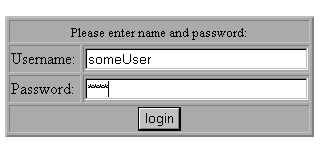
\includegraphics[clip,width=0.4\linewidth]{pics/modules/48}
\end{center}
\caption[Personalization Pic 1 ]{Personalization Pic 1.}
\label{Password}
\end{figure}

The method returns the login name when the login was successful,
otherwise it returns a {\class CmsException}. The exception can be captured and
an appropriate error message displayed to the user.{figure~\ref{HelloUser}}

\begin{figure}
\begin{center}
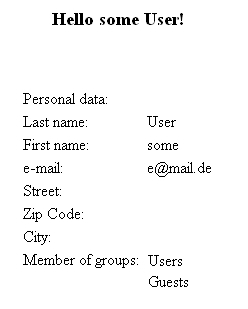
\includegraphics[clip,width=0.4\linewidth]{pics/modules/49}
\end{center}
\caption[Personalization Pic 2]{Personalization Pic 2.}
\label{HelloUser}
\end{figure}

\begin{java}
...try \{\\
cms.loginUser(name, pass);\\
\jtabc                ...\\
\jtabc                templateSelector = "logged\_in";\\
\jtaba          \} catch (Exception e) \{\\
\jtabc                e.printStackTrace(System.err);\\
\jtabc                template.setData("setaction", "send");\\
\jtabc                templateSelector = "error";\\
\jtaba        \}\\
\end{java}

The user data is accessed via the methods of the {\class CmsUser} class. Several
get methods can be used to fetch user data such as the first and last
name and the e-mail address. A hash table is used to store additional
information, which defined and passed using the methods:



\begin{java}
public setAdditionalInfo(String key, Object obj);\\
public Object getAdditionalInfo(String key);\\
\end{java}



This is the output of the above logged in example user:

In addition to the name and e-mail address, additional information
fields can be used to capture use-related data that is essential to
create personalized content.

An alternative to using the additional information hash table would be
to customize OpenCms' user management. Since OpenCms is an open source
project everyone can modify the user management by inheriting the
existing classes or extending the existing ones with additional features.

